

\section{Background}\label{sec:visbg}

In deciding on the best method in which to portray scientific information we must first look at how our ability to understand comprehend information has changed over time. This section looks at now an increase in neocortex size proves pivotal to the sudden rise to power sapiens experinced as a species, and in turn the development of language and visualisation in the context of information transfer. 

In nature many animals are rely on the propagation of DNA to encode important information essential to their survival. Examples of these are seen in hives (where an insects role is defined by its genetic composition), or in Oscines (songbirds) which have an inherent predisposition to learn species specific songs, \citep{modelingpythonbees,genomics,birds,birdsongs,sapiens}.
In sapiens, the vast and varied nature of the information we are required to process makes this process highly impractical. Instead we develop a predisposition to learning language at an early age. Such a skill allows for the effective communication of ideas, conditions and dangers between a large number of people\footnote{Several studies, exploring the ratio of the neocortex to the rest of the brain, suggest that the number of relationships a human can successfully monitor is limited to ~150. It is suggested that ideas of gossip and common metaphysical beliefs are the reason for this \citep{sapiens,neo,gossip}. This limit is still seen in social networks today \citep{social}.}.

Howevever since communicatory patterns are limited to only the people they have been taught to, problems of differing language and dialect greatly reduce the amount of information which may be passed between groups or tribes. One way to overcome falls in the use of pictographs, a form of visualisation colloquially known as cave paintings (e.g. \autoref{cave}) which complements the sapien ability to both detect shapes and spot patterns within nature\footnote{It has been found that 10,000-year-old pictographs show hints of a common cultural background between spatially different groups of humans \citep{cave}.}. As communities increased in size, problems of accounting and resource management begin to emerge.




 \emph{REWRITE:
 Until this point an ability to store large amounts of numerical data had not been required by a hunter-gatherer species.} Around 3,500BC, the Samaritans solved this probelm with the creation of a system for coordinating affairs and storing information external to peoples brains. 

This system is that of writing \citep{archaic,beforeCuneiform}. Here quantities and items are depicted using a numerical system of signs and visual system of shapes (cuneiform\footnote{This is often mistaken for hieroglyphics. Although both are forms of logographic script, hieroglyphs are restricted to the ancient Egyptian sociolinguistic context. }). This external method of storing information, coupled with visual representation, allowed for a an effective and intuitive way for us to apply the pattern recognition and analytical parts of our brain whilst reducing the cognitive load by breaking up the problem into managable parts. 


\begin{figure}[H]
         \centering
         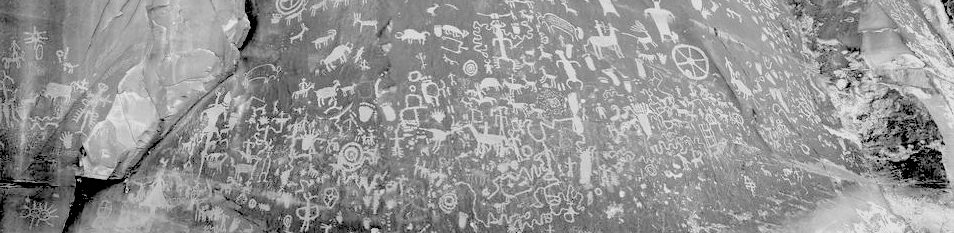
\includegraphics[width=\textwidth]{figures_c1/newspaperrock.jpg}
        \caption{\textbf{An example pictograph:} a 2000 year old petroglyth in Utah titled `Tse Hane' (rock that tells a story). Source:
        \citep{newspaperrock} }
        \label{cave}
\end{figure}

Throughout history, we have continued to apply this system of intertwining data information with visual artifacts to enable people to cope with the complexities of the infomation provided, \citep{tufte}. In the remainder of this chapter the use of visualisation as a means of enchancing the readers ability to understand the large-scale complexities of the chemistry within the troposphere shall be explored. 


\textbf{A note on terminology}
Although the word \emph{species} refers to the biological definition within this section, any further reference throughout this thesis refers to the chemical definition instead. 





%-----------------------------------------------


\section{Introduction}
The term `Big Data' originated in the mid-1990s, appearing in several job adverts and a slide deck by Jon Mashey the chief scientist at Silicon Graphics (SGI), \citep{slidedeck,bigdataorigin}. This term is used as a way to describe the ever-increasing amount we can generate each day. Such phenomenons are seen in anything from the growing number of websites to the number of reactions within a near explicit gas-phase chemistry mechanism, \autoref{fig:webmcm}. Coupled with the ability to collect large amounts of data is our requirement to analyse and understand it. This has commonly be done through the use of visualisation, a topic in which careful consideration must be made to ensure the correct information is conveyed \citep{kirk}. In a paper on mining big data, \citep{bigdatamine} explains that the main task of Big
Data analysis is on deciding how to visualise the results- simply its size introduces complexity in uncovering a user-friendly method to represent the information required. 

Although graphical representation has been an integral part of the data comprehension process, it is only relatively recently (1990's) that it is recognised as a research field \citep{ch6}. Even though we are not explicitly dealing with `big' data, the number of species and reactions within the troposphere are still sufficiently large such that many of the same problems still exist. It is for this reason that this section\footnote{and consequently much of this thesis}, will explore topics such as considerations that need to be made before selecting a visualisation (\autoref{sec:visdes}) and the methods we can use to represent the complex relationships within the atmospheric chemistry domain (\autoref{sec:visrel}). 

\begin{figure}[H]
     \centering
         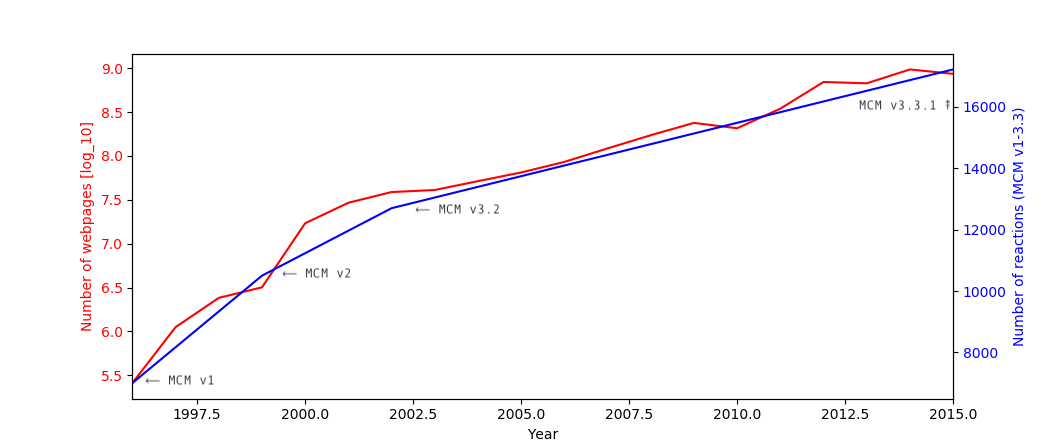
\includegraphics[width=.95\textwidth]{figures_c1/webmcm.png}
         \caption{\textbf{Growing trends in data.} This figure shows the change in the number of websites ($\log_{10}$ normalised) between 1996 and 2015 in red, and the changes of species for the number of reactions within the master chemical mechanism for versions 1 to 3.3.1 - This is introduced later on. \emph{Note: The two lines are here to illustrate the growing trends between the subjects and are not incomparable due to their differing scales.}  Source: \citep{webstats,mcmhist}}
         \label{fig:webmcm}
\end{figure}


\subsection{Visualisation Design}\label{sec:visdes}


New ideas are developed and refined through an iterative process of cognition and discussion with other researchers\citep{ch7}. 
As we are constrained by our experience and knowledge, novel ideas often consist of an amalgamation of many existing concepts \citep{wingedhorse,goodideas}. \citep{shapinginfo} suggests that the process of understanding a visualisation depends heavily on the interaction between the user's internal knowledge and experience with the images and ideas depicted within the visualisation. This means that the careful selection of content and medium (of presentation) can directly influence what a reader takes away from the graphic.

Knowledge and experience dictate how we may perceive new data. This means that a data visualisation designed to be relate-able in content and representation to a reader will have a much higher chance in conveying the correct information successfully. As a consequence of this, the interface between quantitative science and the user (i.e. the visualisation) will have a higher knowledge transfer or throughput. Here two visualisation design considerations (storytelling and metaphor selection) are discussed. 



\subsubsection{Storytelling}\label{sec:storytelling}

Storytelling is commonly used to highlight the process of cause and effect. It has applications in the education for both the explanation of scientific concepts (\citep{marsstory}) and the dangers of the world (fables such as Little Red Riding Hood and Goldilocks teach the dangers of speaking to strangers and the importance of respecting personal property). As human life is subject to the conditions of the `arrow of time', the inherent familiarity of linearly consequential events make the narrative a great way to inform the reader of new (unseen) concepts. Such methods are not limited to the education of young children, but also allow for the understanding of real-world events through the use of dreams, media and the news \citep{storyanimal,dream}. 

With the use of a narrative, a visualisation can educate the user, providing them with a level of prerequisite knowledge that then enables them to draw their own (guided) conclusion. In exploring how people interperate visualisation, it is seen that readers apply a visual routine to create a narrative and compare values within a graph, \citep{eyestory}. This emphasizes the importance of designing a visualisation in such a way that the user is `guided' through the correct narrative. The question-answer cause-effect structure not only satisfies the inquisitive nature of the human species, but it also educates the reader to the events which led to a certain conclusion. It is this process that makes `storytelling' an effective method of communication to a non-expert audience \citep{nonscientific}.


\subsubsection{Metaphor Selection}
In addition to storytelling, the use of suitable metaphor is also important in designing a visualisation capable of appealing to the users' knowledge and experience.  Much like the use of narrative, metaphors have infiltrated our everyday lives. These range from the morals presented by fables, to the concept of money and belief to govern everyday life through the inter-subjective\footnote{The inter-subjective is something that exists within the communication network. It allows a fictional idea, such as a limited-liability company, to exist as a real physical entity with a bank account and subject to laws. } \citep{sapiens}. 

In selecting a suitable metaphor for a visualisation we often have three options. These are natural, man-made and composite. 

\paragraph*{Nature-Inspired}
Inspiration for a metaphor can come from a range of sources. The most effective of which, often have objects of events which are universal and inherently familiar to all readers. The most widely used of these are nature-inspired metaphors. 
Such metaphors do not only guarantee a basic level of item comprehension but also have an aesthetically pleasing
quality and familiarity to the visualisation components. 

Examples of these may be the use of ice and water to symbolise glacial melting, using trees to represent the binary decision tree of a random Forrest (\autoref{fig:1tree}), or rings within a trunk cross-section (\autoref{fig:trunk}) to show changes in conditions over time. The main benefit of using natural metaphors is the low learning curve required to understand them. 


\begin{figure}[H]
     \centering
     \begin{subfigure}[b]{0.495\textwidth}
         \centering
         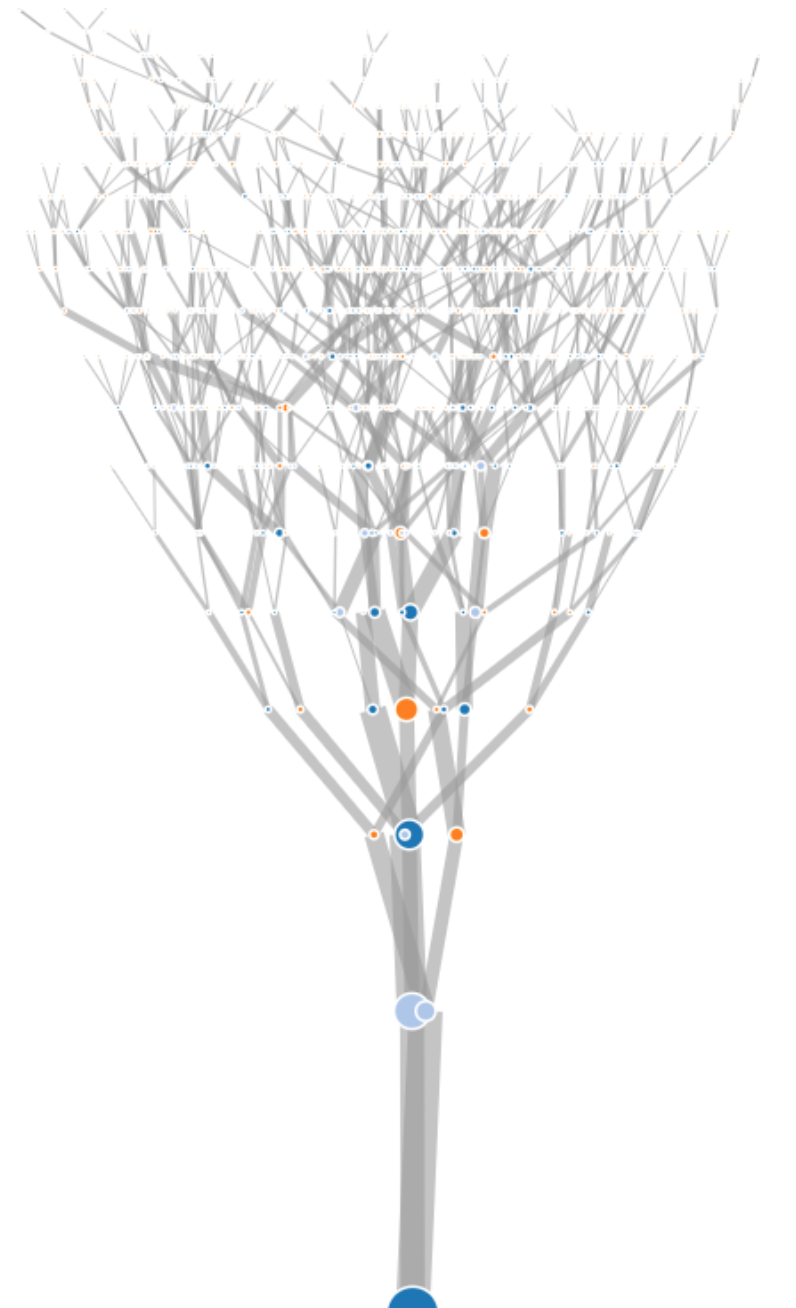
\includegraphics[width=0.8\textwidth,height=\textwidth]{figures_c1/tree.png}
         \caption{Single Tree (coloured leaves)}
         \label{fig:1tree}
     \end{subfigure}
     \hfill
     \begin{subfigure}[b]{0.495\textwidth}
         \centering
         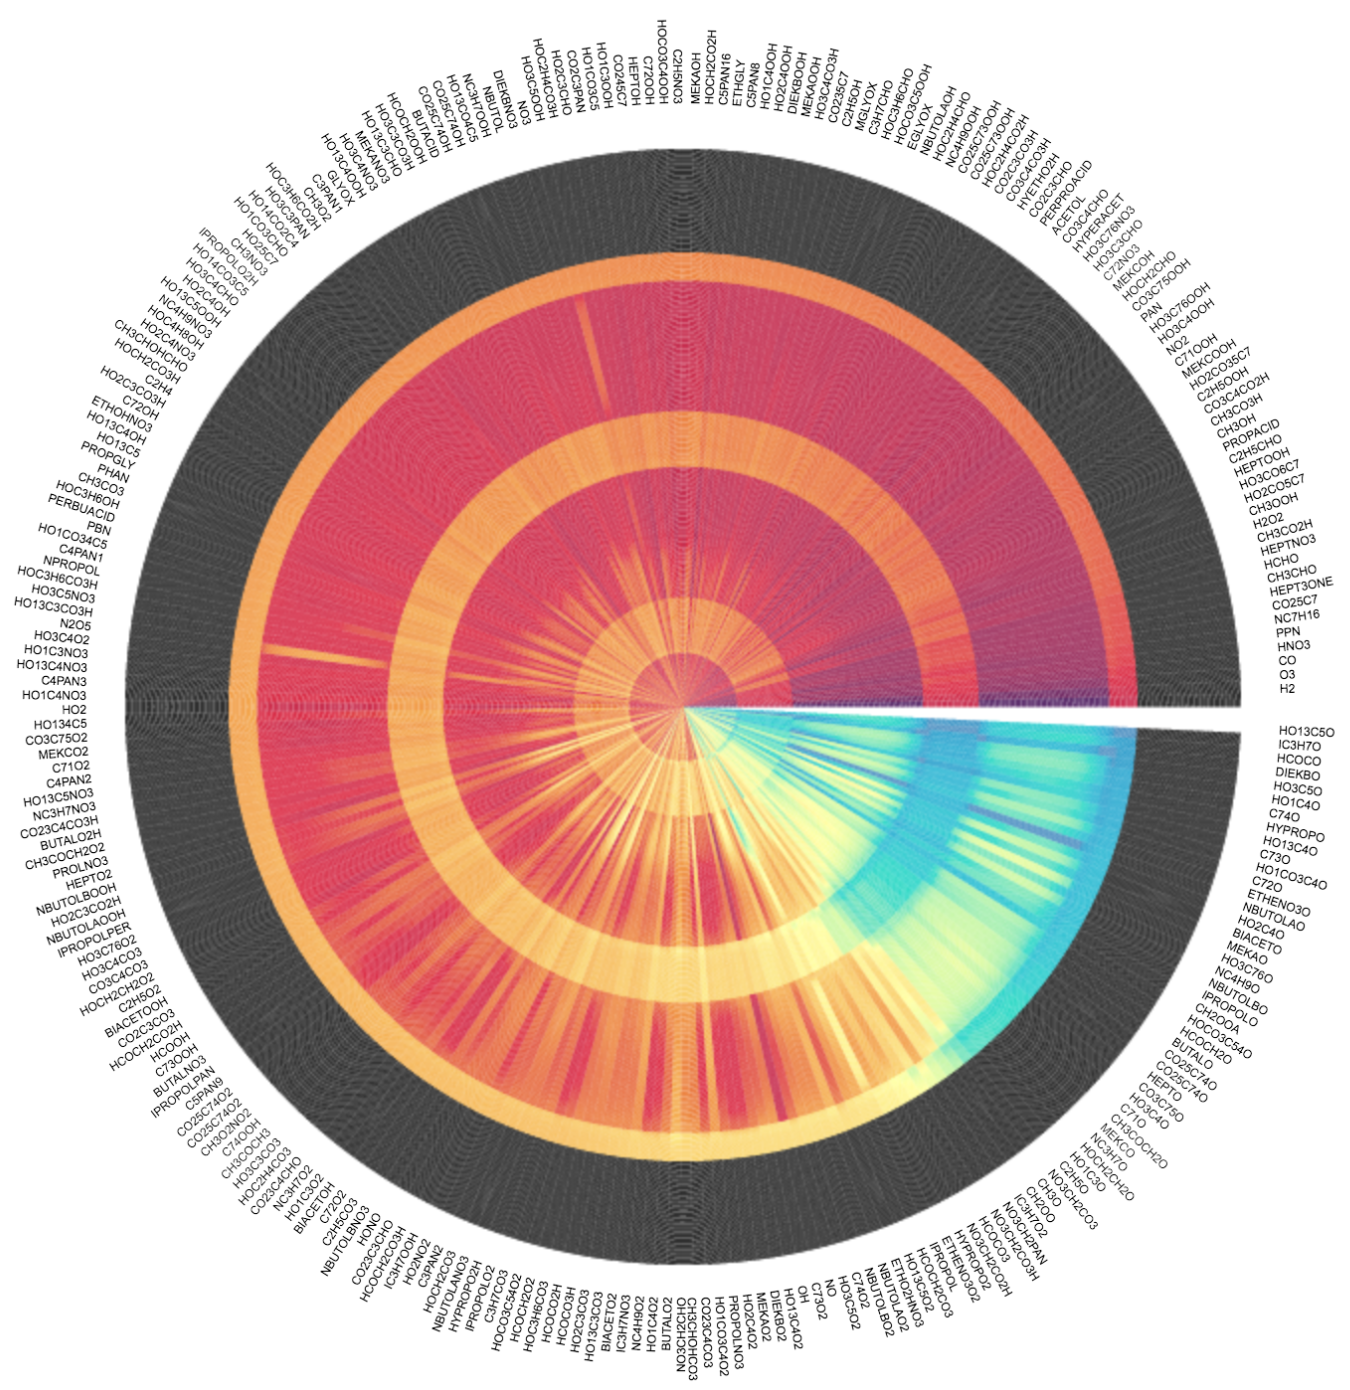
\includegraphics[width=\textwidth]{figures_c1/trunk.png}
         \caption{Complete tree trunk}
         \label{fig:trunk}
     \end{subfigure}
     
    
        \caption{\textbf{A collection of tree-based visualisations.}
         (a) shows the decisions made on a tree within a random Forrest. Node/Leaf colour represents the property which is being decided, whilst node and branch size are symbolic of its importance (Larger leaves/branches are naturally stronger and more important).\\
          (b) is a radial plot in the shape of a tree trunk. Much like that of a real tree, time is shown across the radial direction, starting at the origin. The colours represent the net flux of a series of species from a chemical simulation. Much like in a tree, large scale events produce a change in the ring colour (these are seen in avalanches and tsunami struck forests) - in this case, the abrupt changes are due to the diurnal cycle.}
        \label{fig:trees}
\end{figure}


\paragraph*{Man-made}
Similar to nature, another similarity between many readers would be their familiarity with the urban environment. Metaphor inspiration from man-made objects such as objects, buildings often contain characteristics of symmetry and manual/mechanical design. These allow the user to interpret any features presented using their pre-existing knowledge about an object. The most famous example of this is Henry Beck's tube map (1933) \citep{beck} where stations are positioned at 0,90 and 45-degree angles. This provides a clearer representation, much like a road map than the conventional space-specific location of each station. Although other designs, such as a concentric one, \citep{circ}, have been attempted, adaptations of Beck's design are still being used in the present day due to their intuitive nature. 
% 
% Similar techniques have also been applied in the field of cartography where, for example, the mercator projection, \citep{mercator} aids navigation, whereas the equal area projection is more suited to size comparison.
% 
%

\begin{figure}[H]
     \centering

         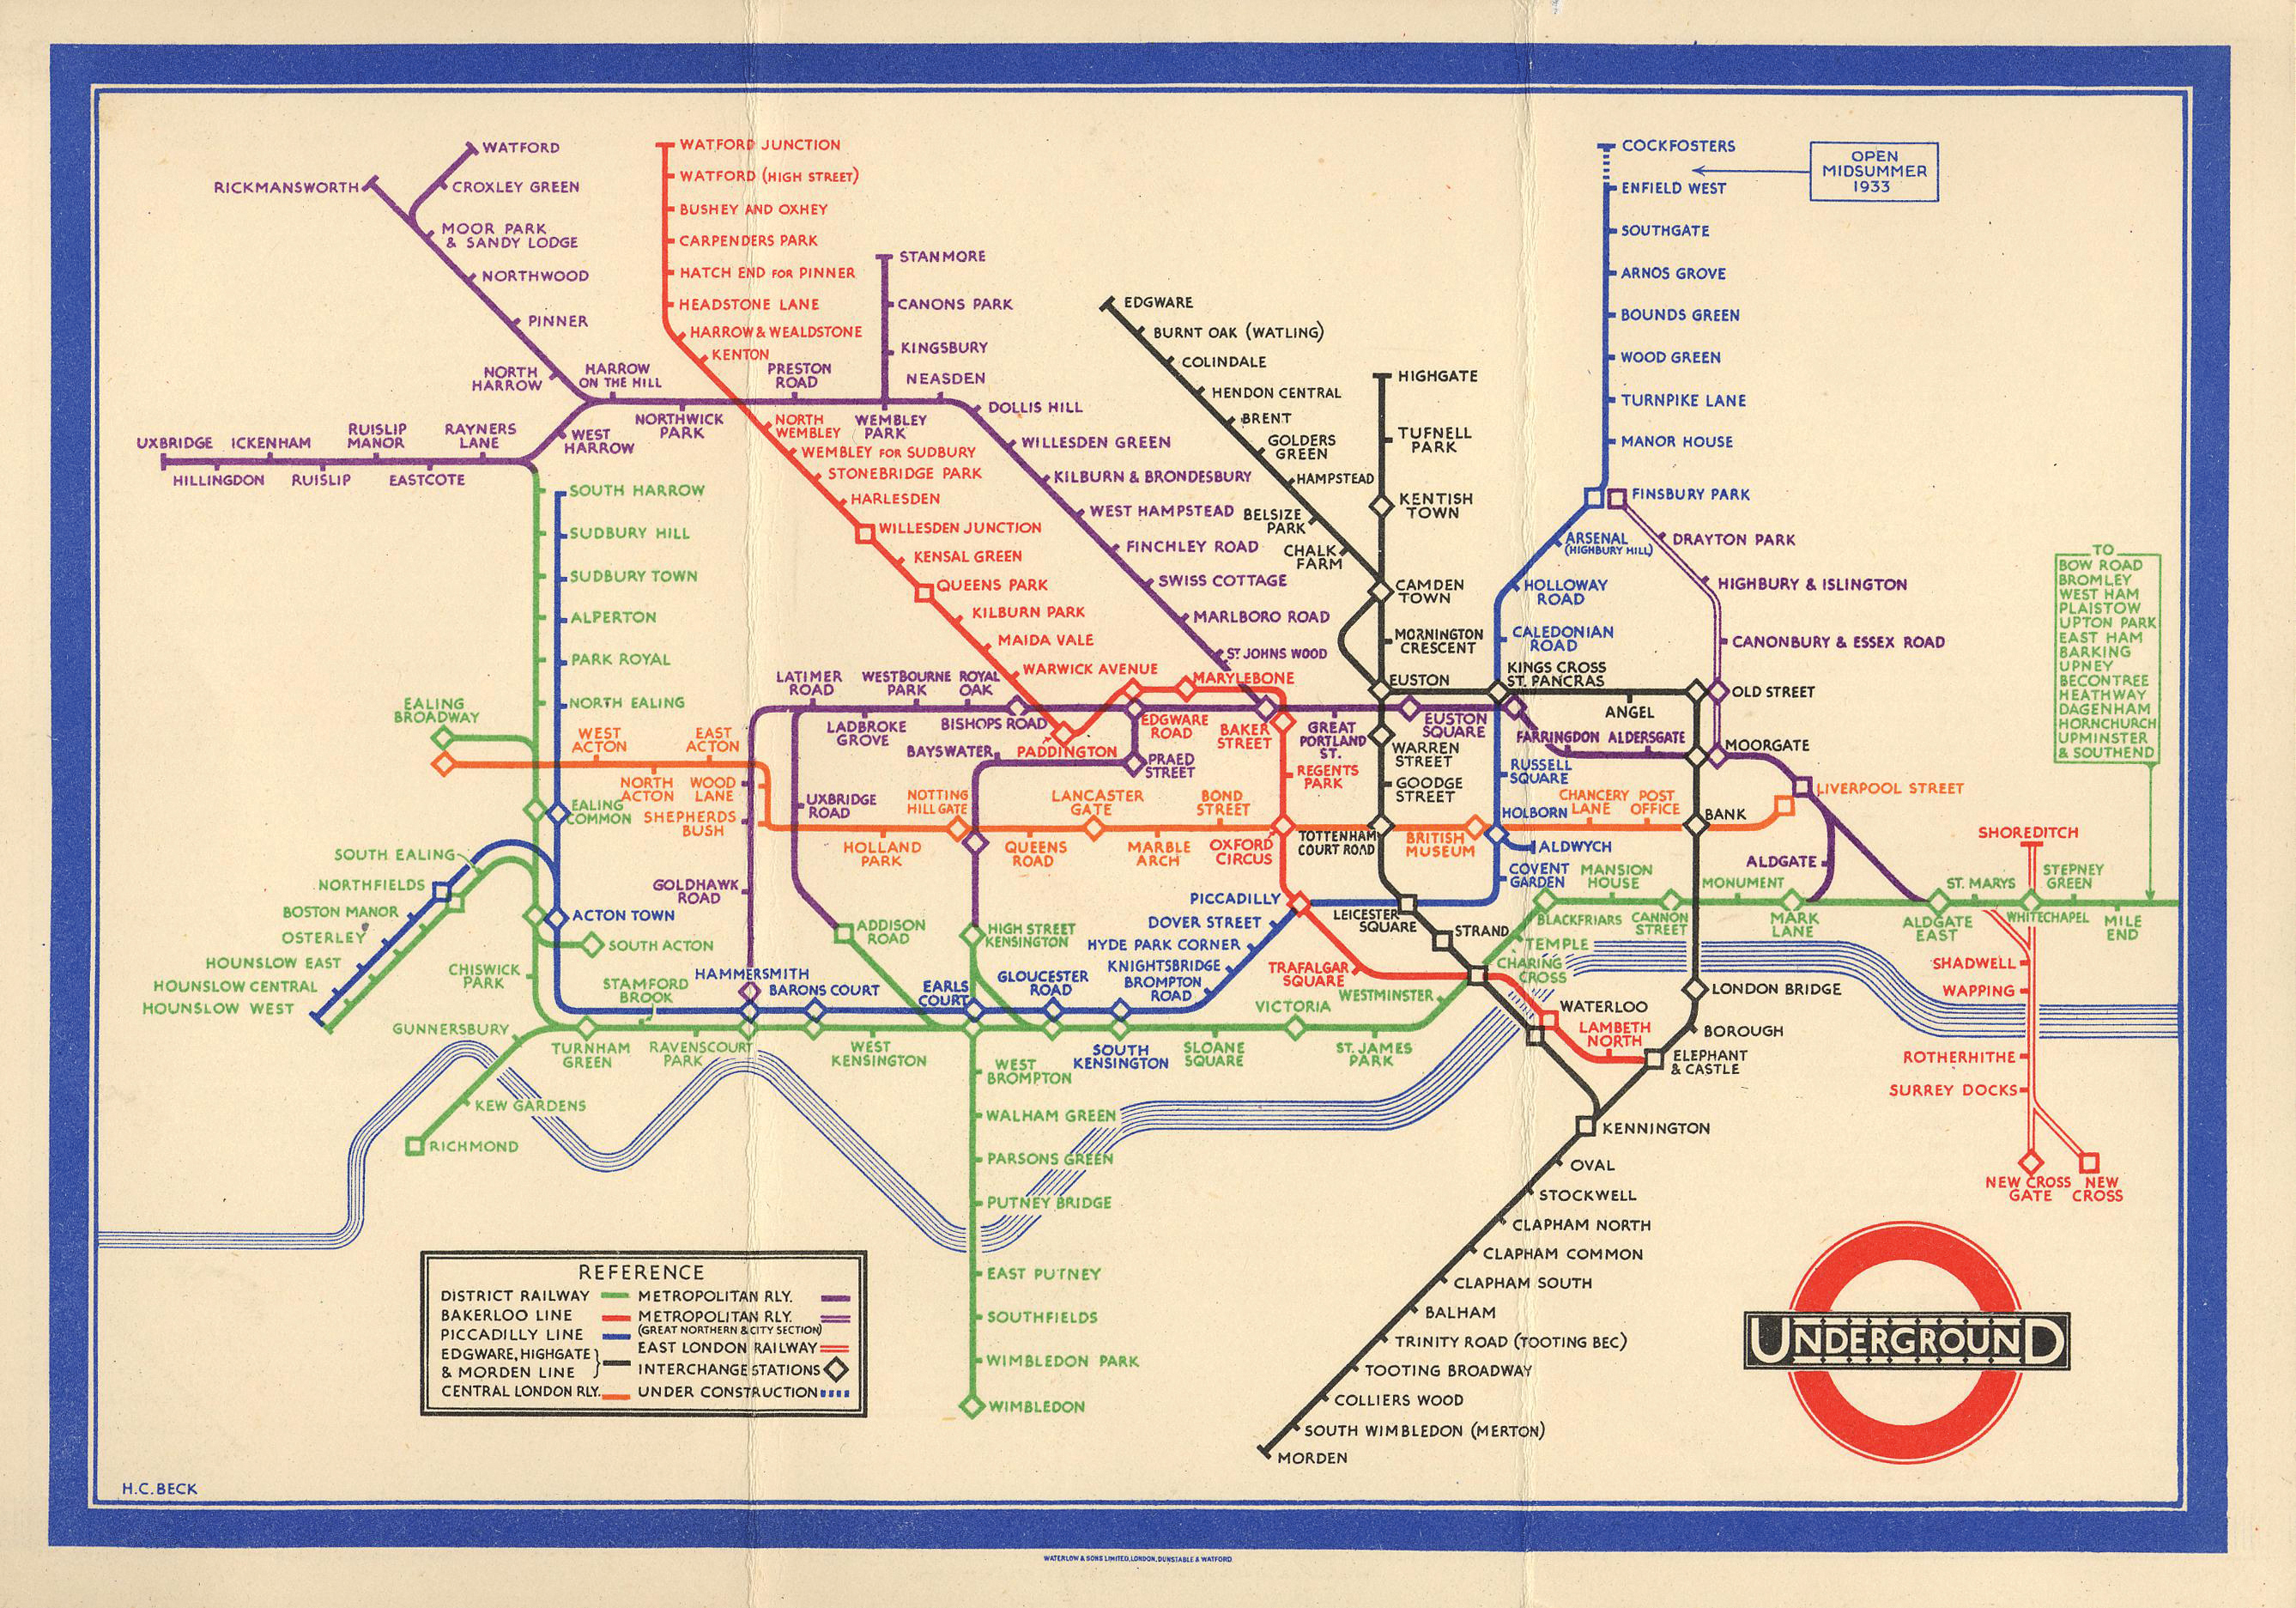
\includegraphics[width=.495\textwidth]{figures_c1/Beck_Map_1933.jpg}
         \vspace{5mm}
         
         \caption{\textbf{The classic tube map design.} Source: \citep{beck}}
         
         \label{fig:beck}

\end{figure}

\paragraph*{Composite}


Sometimes ideas may be combined to provide a composite metaphor. The classic example of this is seen in much of greek mythology with the concept of Pegasus. Here although we are familiar with the concepts of both wings and a horse, no one has encountered such a creature - yet we can assume the implications of its existence.
Here the inspiration of new designs often stems from many different sources which are confluent and refined through the use of sketches and doodles \citep{fds}. 

Similarly, it is possible to drive inspiration from a range of sources: natural, anthropogenic, other visualisations etc. 
Such techniques allow for the creation of xenographics, with the most famous example falling under the combination of a `pizza/pie chart'\footnote{There is a good amount of literature that suggests these are far from optimal methods of representing data. } with a bar chart to create a radial plot in \autoref{fig:nightingale} - A novel representation which helped establish the methods of modern-day nursing by Florence Nightingale. 
Overcoming the problems presented by these composite designs involves a level of lateral thinking to produce a simpler, more effective, user-visual metaphor interaction \citep{shapinginfo}. 



\begin{figure}[H]
     \centering
         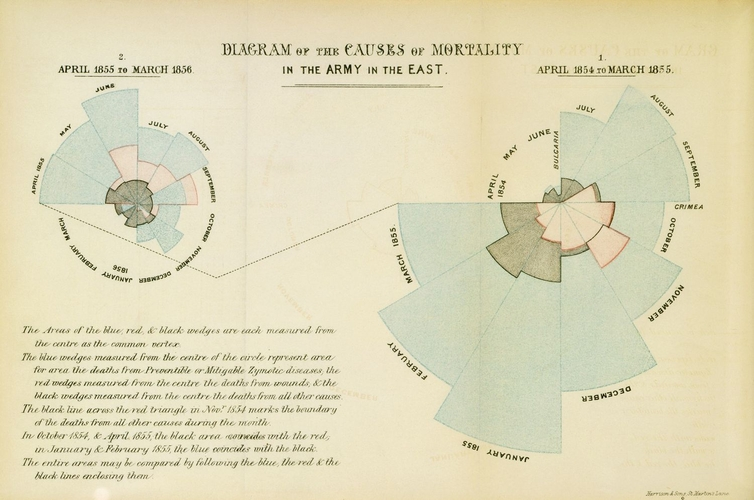
\includegraphics[width=.75\textwidth]{figures_c1/nightingale.jpg}
        \caption[Caption for LOF]{\textbf{A (stacked) Radial bar-chart showing the causes of mortality in the British army}\protect\footnotemark , \citep{nightingale}.}
        \label{fig:nightingale}
\end{figure}
% Footnote CAPTION hack! 
\footnotetext{Also known as the Nightingale Rose or Coxcomb plot.}




\paragraph*{Domain Specific}




Composite designs are not constrained to the combination of different metaphors. In specialised roles, it is common to find visualisations which draw on pre-existing knowledge either about the content of the figure. Although this involves an additional learning curve before information about the topic can be extracted, once this is obtained, the wealth and complexity that is portrayed by a single visualisation drastically increases. Two of the more common examples where prior knowledge is required to read a plot are connected scatter plots\footnote{ Occasionally known as snail trail chart (R users seem to like re-inventing the wheel). } and Tephigrams. 

\textbf{T-$\phi$-grams (Tephigrams)} are defined from their axis of temperature ($T$), entropy($\phi$) are used in the field of meteorology and weather forecasting. The combine grid lines for constant temperature and pressure, as well as allowing the user to calculate the equivalent potential temperature for saturated air parcels and the saturation mixing ratio concerning plane water surface, \autoref{fig:tefidesc}. This provides a good example where both scientific knowledge and ability to read the diagram are required to obtain meaningful information from it. 

\begin{figure}[H]
     \centering
     \begin{subfigure}[b]{0.4\textwidth}
         \centering
         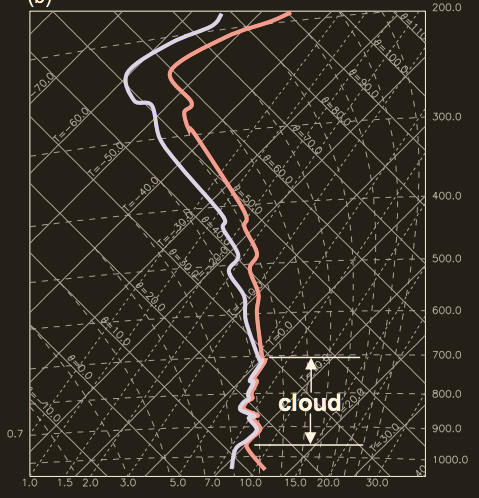
\includegraphics[height=1.325\textwidth,width=\textwidth]{figures_c1/tephiuse.png}
         \caption{A tephi diagram}
         \label{fig:tephidiag}
     \end{subfigure}
     \hfill
     \begin{subfigure}[b]{0.59\textwidth}
         \centering
         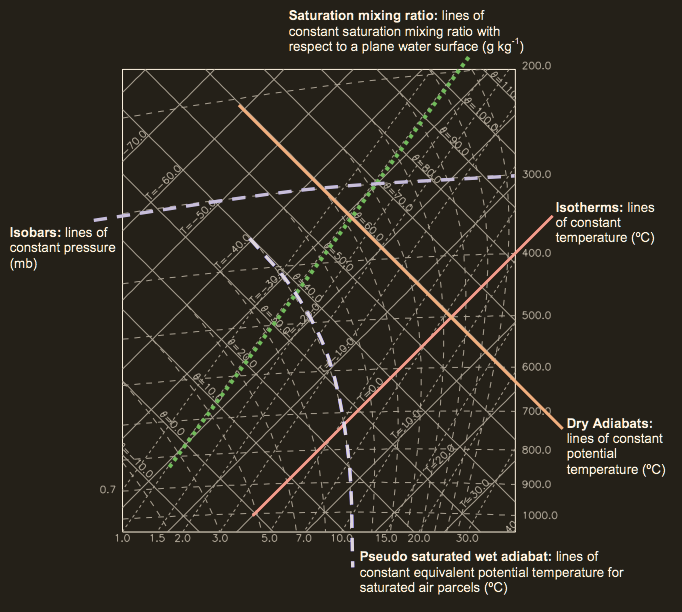
\includegraphics[width=\textwidth]{figures_c1/tephidescribe.png}
         \caption{Description of each axis on the tephi diagram. }
         \label{fig:tefidesc}
     \end{subfigure}
        \caption{\textbf{Two T-$\phi$-gram plots.} An example of the T-$\phi$-gram data (a),  and instructions on how to interperate it (b). Source: \citep{tephi}}
        \label{fig:tephi}
\end{figure}


\textbf{Connected scatter-plots} are useful in representing the temporal changes of correlation between to items. These are particularly useful in the field of economics due to their ability to highlight the different trends that can occur over time. \autoref{fig:conscat} shows how the number of vehicle-related fatalities changes with the number miles driven. In this situation, a simple $x-y$ plot may highlight a decreasing inverse relationship between the number of fatalities and the miles driven per capita over time, but lose some of the many features presented by the additional dimension. 


\begin{figure}[H]
     \centering
         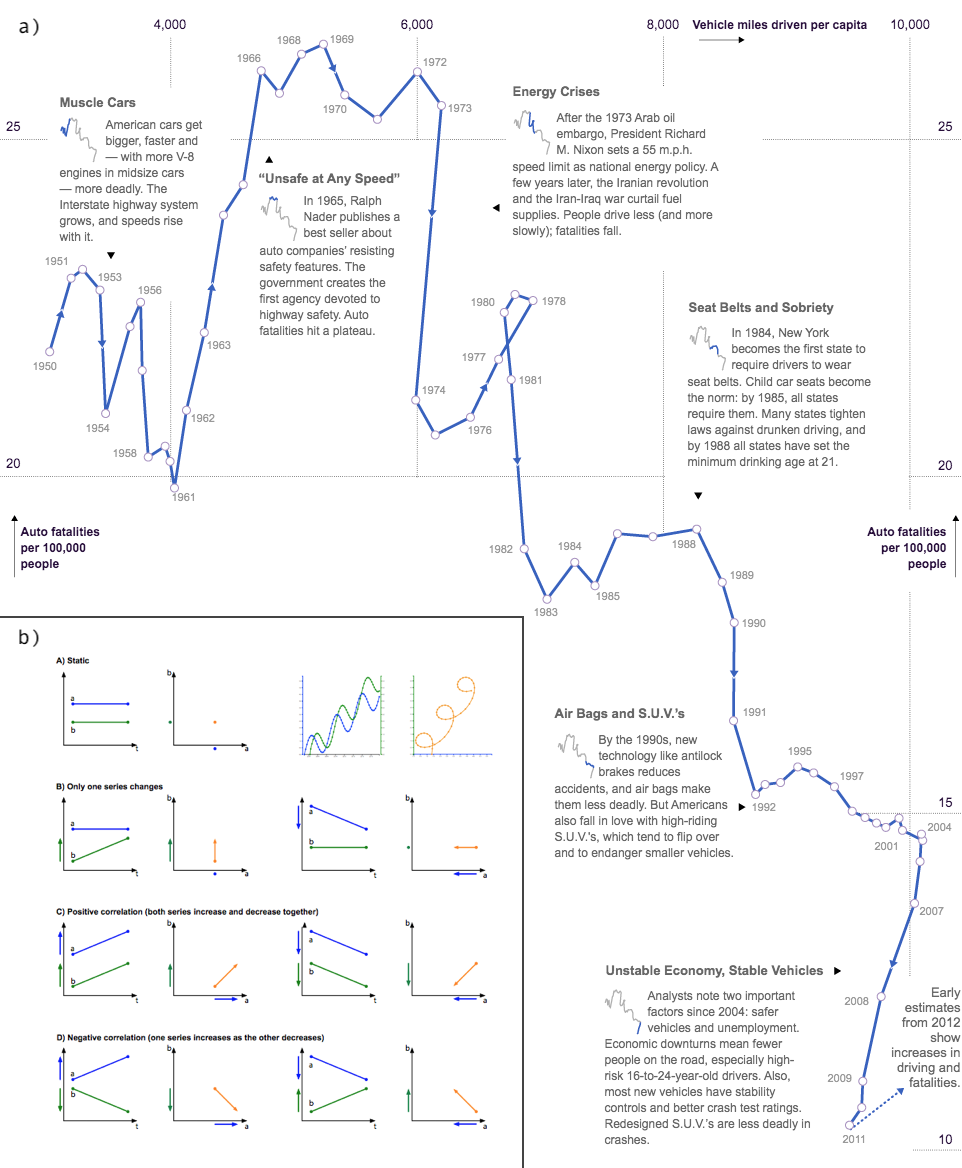
\includegraphics[width=\textwidth]{figures_c1/connectedscatter.png}
        \caption{\textbf{Examples of connected scatterplots} (a) A connected scatter-plot comparing the the number of vehicle related fatalites with the number miles driven per capita \citep{conscat}\\
        (b) a plot showing how the corellation of two spatial variables are transformed from a classical scatter/line plot into a connected scatter-plot \citep{defconscat}. }
        \label{fig:conscat}
\end{figure}
\newpage




\subsection{Visualising Relationships}\label{sec:visrel}

Discerning important relationships is a vital part of both science and pattern recognition. Even in storytelling (\autoref{sec:storytelling}), we see readers trying to piece together a relationship between events, actions and outcomes. It is for this reason that we shall explore the different ways in which we may visually represent relationships within science. To do this we first define a dataset (\autoref{sec:dataset}) - in this case, this is the master chemical mechanism (described below). We then proceed to identify a variety of different visualisation methods, before expanding on a particular style of visual analytics in \autoref{sec:va}.

\subsubsection{The Dataset}\label{sec:dataset}
Since our topic of interest lies in the representation of chemistry within the atmosphere, we take a set of first-order ordinary differential equations and rates designed to describe
how species react in the troposphere. This set of equations is known as a mechanism. 

The equations we are to use are given by the master chemical mechanism (MCM). This is a near explicit representation of our understanding of the gas-phase chemistry within the troposphere. In its mathematical form, it describes how species are related and at what rate they react. As the aim of this section is to identify features within the chemical mechanism we begin by looking at the mechanisms construction protocol, \autoref{fig:protocol}. In its design, this aims to mimic much of the reasoning and procedures that would be otherwise performed by an analytic chemist. The procedure is semi-automated and follows several iterations starting from a set of primary emitted VOCs. These are run from the protocol to build a set of reactions in which the selected species may undergo. Any new products are then introduced to the procedure until everything has been oxidised to produced carbon dioxide (via CO) and water. This produces the set of near explicit equations which are then used to describe the evolution of chemistry within an atmospheric model. 

\begin{figure}[H]
     \centering
         \centering
         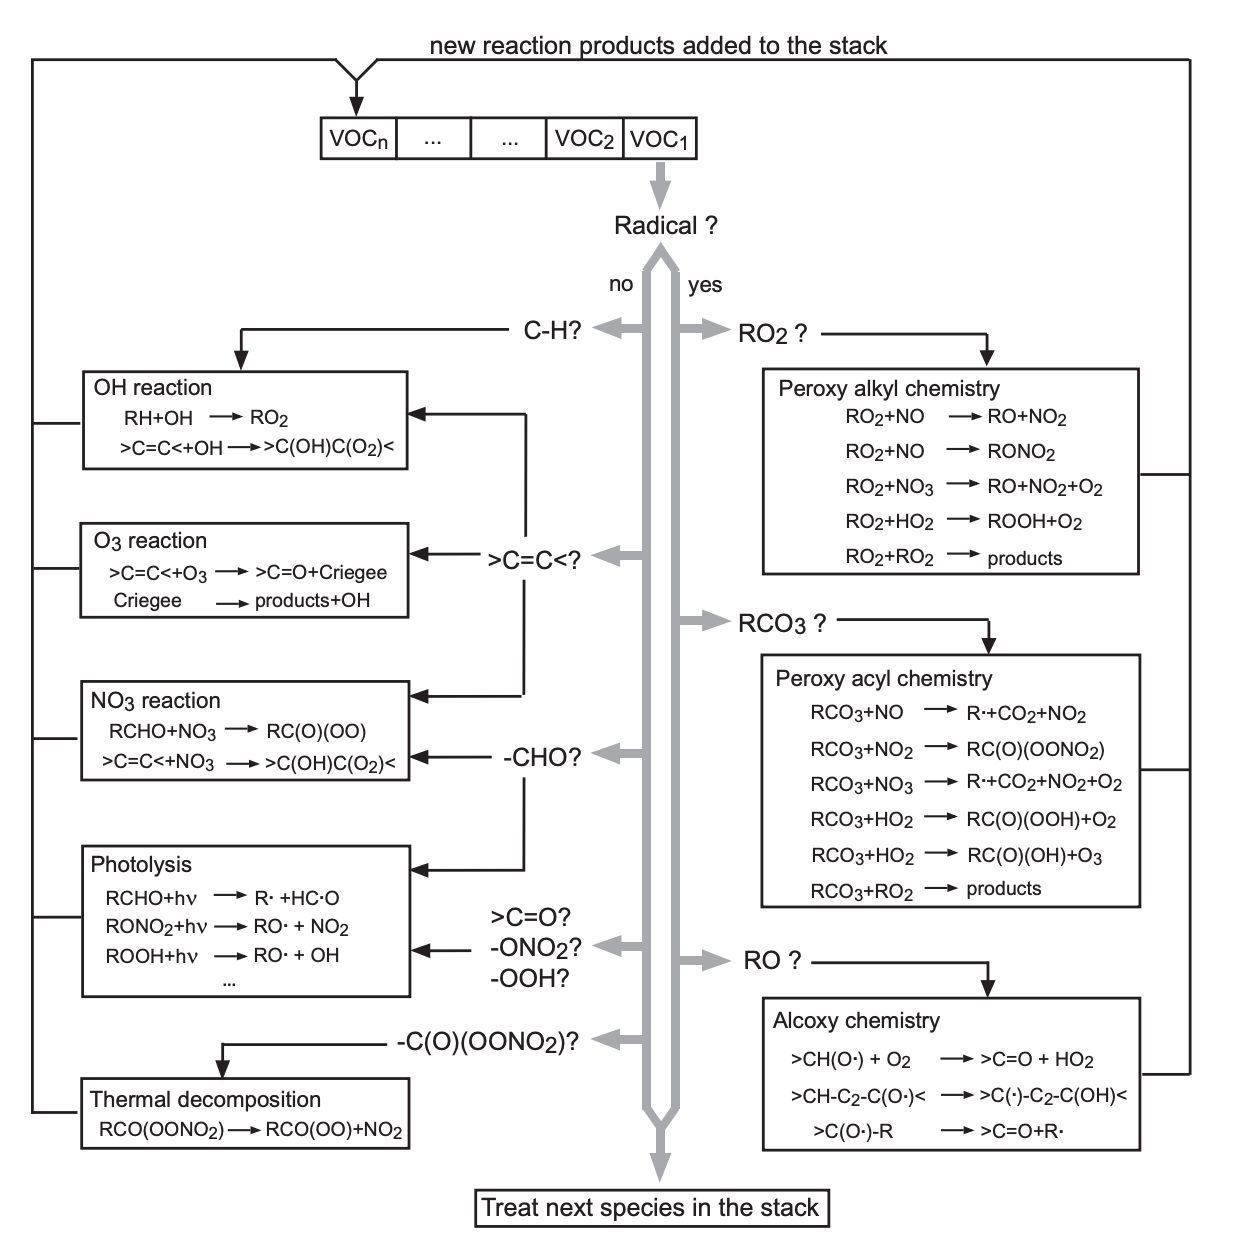
\includegraphics[width=.96\textwidth]{figures_c1/generation.png}
         \caption{\textbf{The generation flowchart used within the MCM.} This shows the process undergone by a new species to generate its products. Any unseen products are then fed back into the flowchart until the entire mechanism has been produced.  Source:\citep{protocol}}
         \label{fig:protocol}
     \end{figure}


\subsection{The social network}
Social network analysis is a type of sociological work (sociometry) that aims to reveal the interweaving and interlocking relations between items or individuals, \citep{socialorigin}. \citep{gossip} argues that the evolution of language as a result of social grooming (gossip), and therefore its adaption for storytelling. It follows that using the social network construct to represent the latent patterns between objects makes use of both our inherent ability to discern complex patterns through the use of storytelling. In trying to depict the relationships between a social network, we employ the use of sociograms. These are a class of visualisations which reveal certain properties of a social network. The following section will look at the extraction of useful information form the relationships within the MCM through the use of several sociograms. 

\subsubsection*{The Chord Diagram}
The chord diagram is a visual sociogram known for its use in summarising the overarching relations within a dense social network,  \citep{chord}. Here arcs are used to represent groups (or a node from a social network graph), and their length corresponds to the percentage of items they contain. Within \autoref{fig:chord} we represent the different routes a species may react within the MCM protocol flowchart in \autoref{fig:protocol}. The figure contains two sets of arcs. These represent the different level of classification of the chemistry - The first (outer) arc represents the split in channels between radical (red) and non-radical (orange) species which further separated into the finer categories within each branch (the labelled inner arcs). The inner arcs again show the probability a randomly chosen reaction on a species will fall under a certain category - if we convert an arc into a segment we have a pie chart of probability. 

\textit{It is worth noting that segment sizes do not represent the number of species undergoing a certain reaction pathway, but rather the percentage of all possible pathways which follow that route. This is because species often undergo a range of reactions, each of which counts as an individual weighting. It is for this reason that even though almost all\footnote{ Except any inorganic species.} contain a C-H bond, does not consume the whole graph. 
}

From this, we see that hydroxy reactions are the most common with C-H bonds being in abundance\footnote{This is seen within the graph layout \autoref{fig:mcmfull}}. We also see that having another type of reaction is also just as probable, with a third of the most utilised branches within the MCM protocol falling under species containing the Carbonyl group. 

Next, we look at the co-occurrence of branches for different species. These are represented using the area of a circle connecting two arcs (a chord). Each chord has two edges connecting two arcs\footnote{With the exception of self loops, although these are addressed below.}. Comparing the width of each chord to its parent arc, it is possible to discern the percentage of items going between these and other branches. Here, for example, we see a roughly even split between species with a hydrogen bond (i.e. all species) and every other group. This suggests an even distribution of reaction types between species. 
This means that in comparing the arc length of each chord, we can visually determine the percentage of group A which relates to its partner group B. Finally it is also possible to determine the number of items in a group which contain themselves. Chemically these are species with multiples of one functional group that undergo a certain reaction pathway more than one time. Although these reactions will be combined within a mechanism (to avoid duplication), their rate would be increased accordingly. 

\begin{figure}[H]
     \centering
     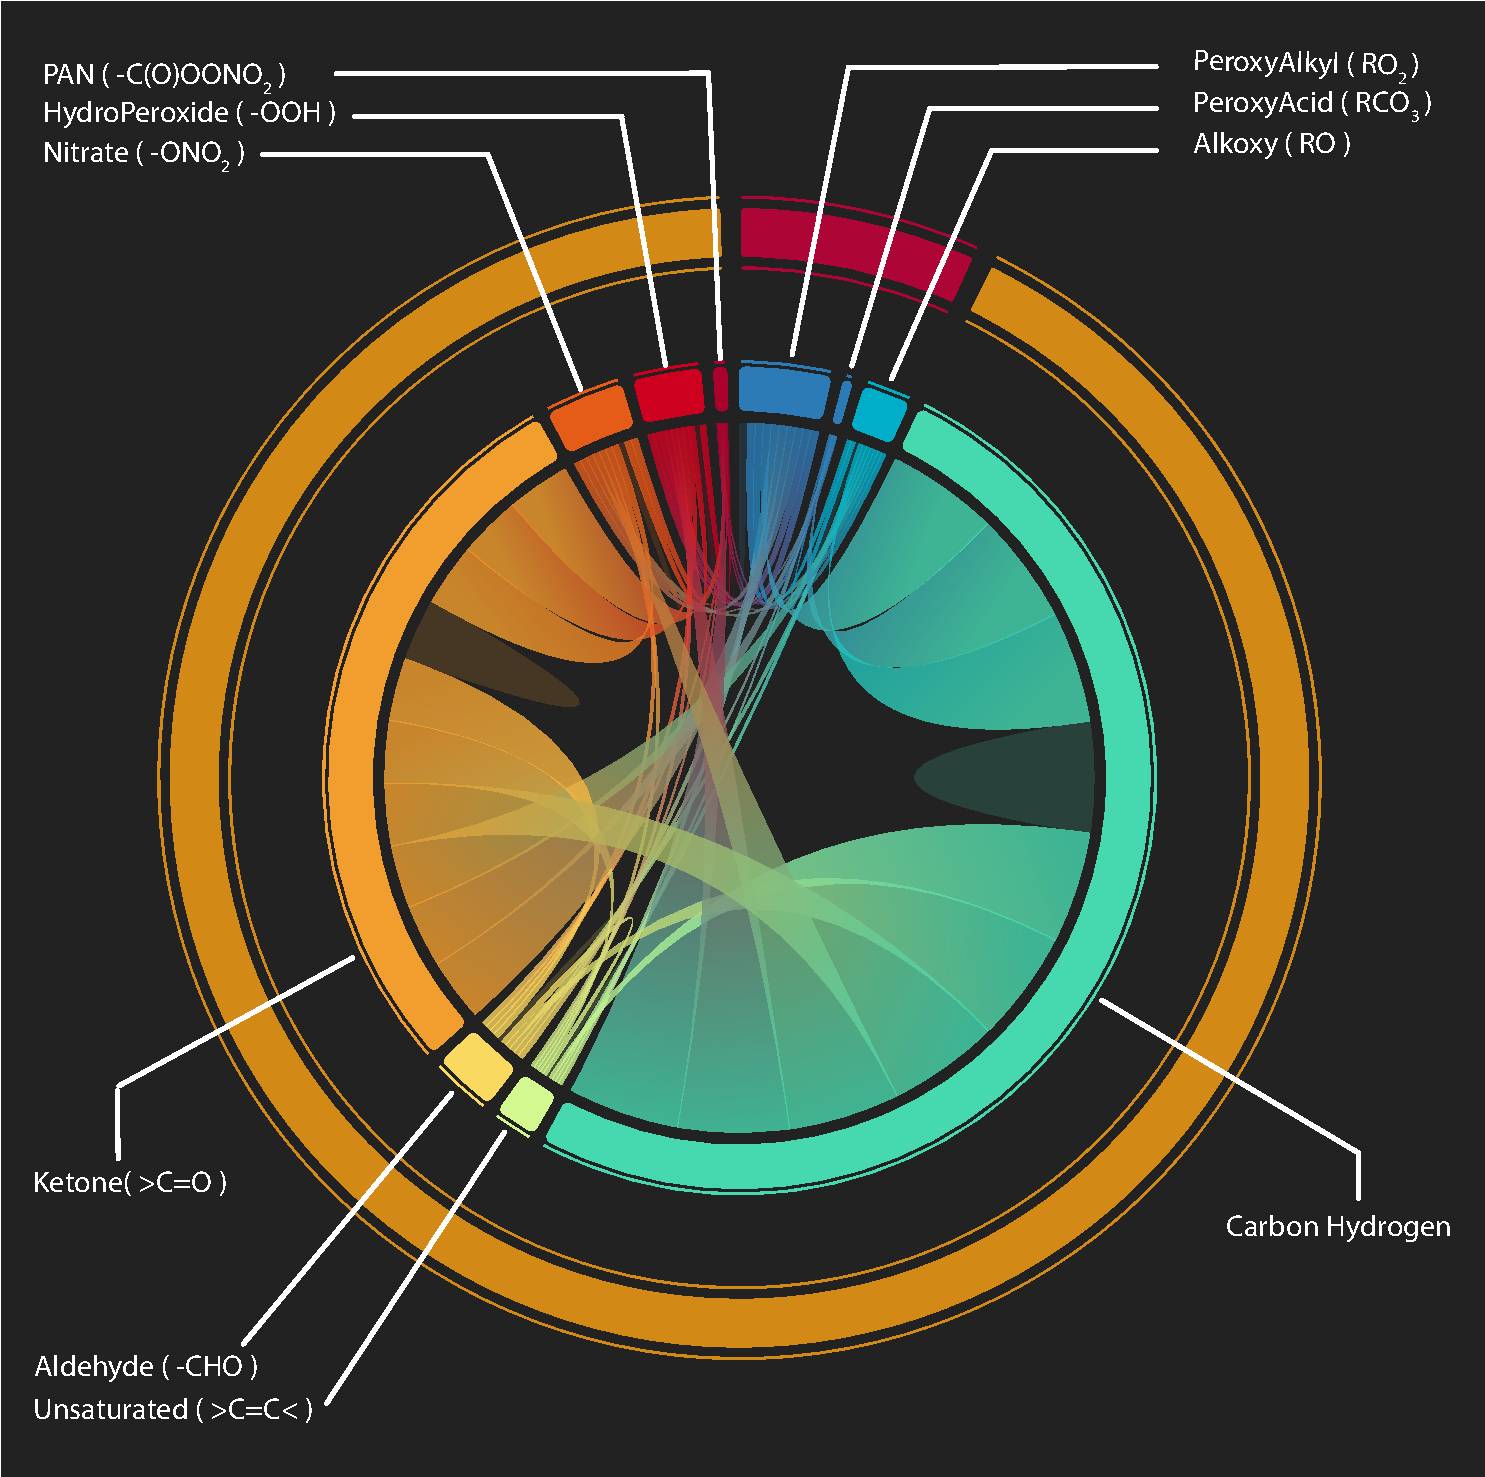
\includegraphics[width=\textwidth]{figures_c1/radicallayermcmgen.pdf}\llap{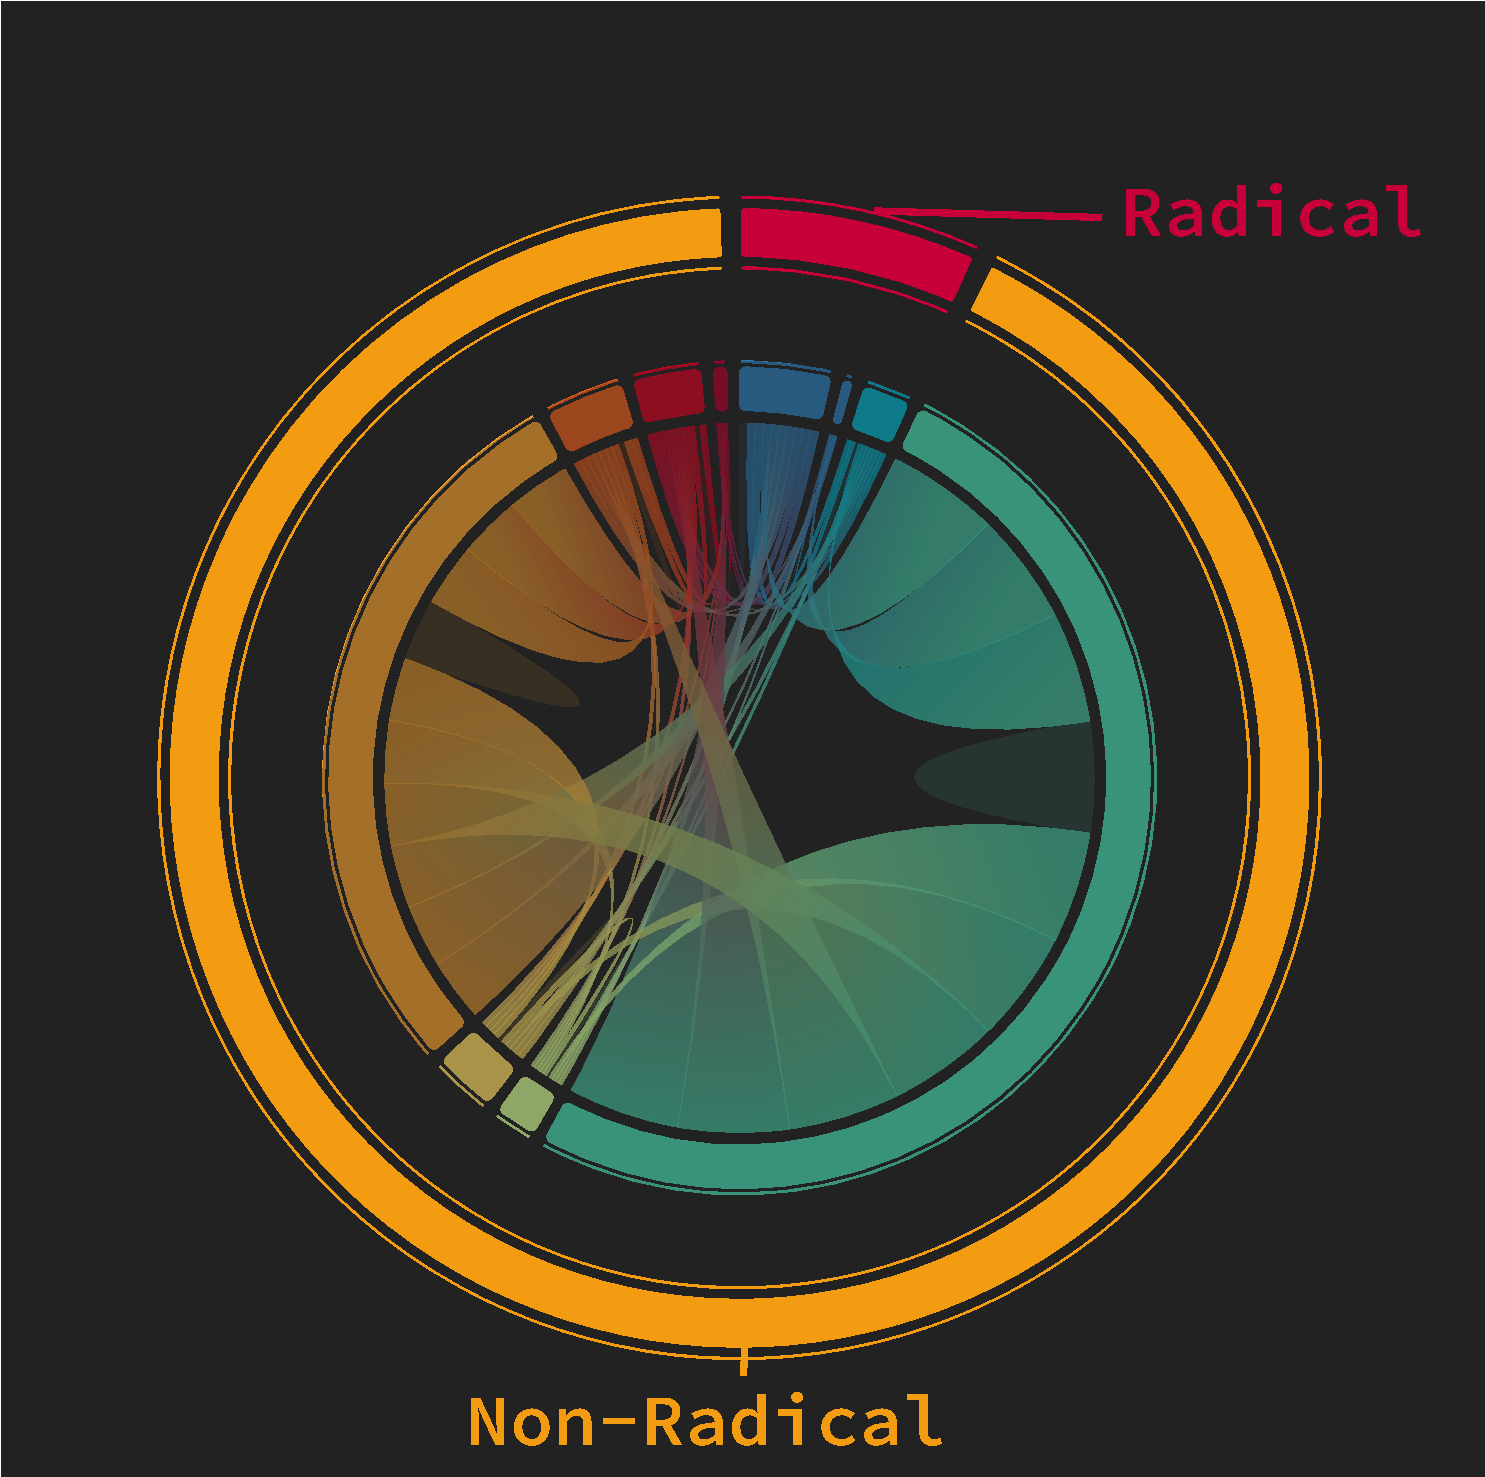
\includegraphics[height=2.5cm]{figures_c1/radicallayersmcmgennamesfinal.pdf}}
        \caption{\textbf{A chord diagram}. This shows the proportional probability a species from the MCM will follow one or more of the paths presented in \autoref{fig:protocol}.}
        \label{fig:chord}
\end{figure}


The chord layout provides an easy way to calculate the percentage of items which contain multiple properties. It requires a relatively low learning curve and is intuitive to those with experience using pie charts (namely the Microsoft Office generation), however, this radial format can sometimes also make it more difficult to read. Special attention needs to be paid to the order arcs are drawn, as with some datasets, certain configurations may obfuscate trends. Finally, the chord diagram requires a certain amount of data munging before its employment. It is due to this that finer details about the system may be lost, especially if there is a corse scale between chord sizes. 










\subsection{Circular Edge Bundling}

Show relationships (see zip on slack)






\subsubsection{Direct representation of the relational matrix}
Relational matrices, also known as the adjacency matrix, are a $n \times n$ square matrix hi-lighting the relationships between items. \autoref{fig:adj} shows the adjacency matrix representing the co-occurrence of characters in the Les-Miserables musical, as provided by \citep{lesmis}. Through ordering, we can achieve a view into the structure of the overall network. Visualisations, such as those in \autoref{fig:adjclust} are often used in the assessment and evaluation of network clustering algorithms since they clearly show the effect modularity has on the diagonal of the adjacency matrix. 


The main downside of this type of visualisation is the sparsity of many graphs. If we take the complete MCM 3.3.1 network, as used above, and visualise it in this manner it will have a density of $5.9 \time 10^{-4}$. This means that for an average $600 \times 600$ pixel figure, only $0.36^2$ of a pixel would be coloured in. And since we are not able to colour only parts of pixels our final plot will remain blank. Methods to circumvent this involve looking at subgraphs, or individual sections interactively or applying composite graph/adjacency techniques such as those presented in NodeTrix, a method for visualising sparse small world networks\footnote{Small world networks are discussed in the following chapter.} \citep{nodetrix}

\begin{figure}[H]
     \centering
      \begin{subfigure}[b]{.49\textwidth}
         \centering
         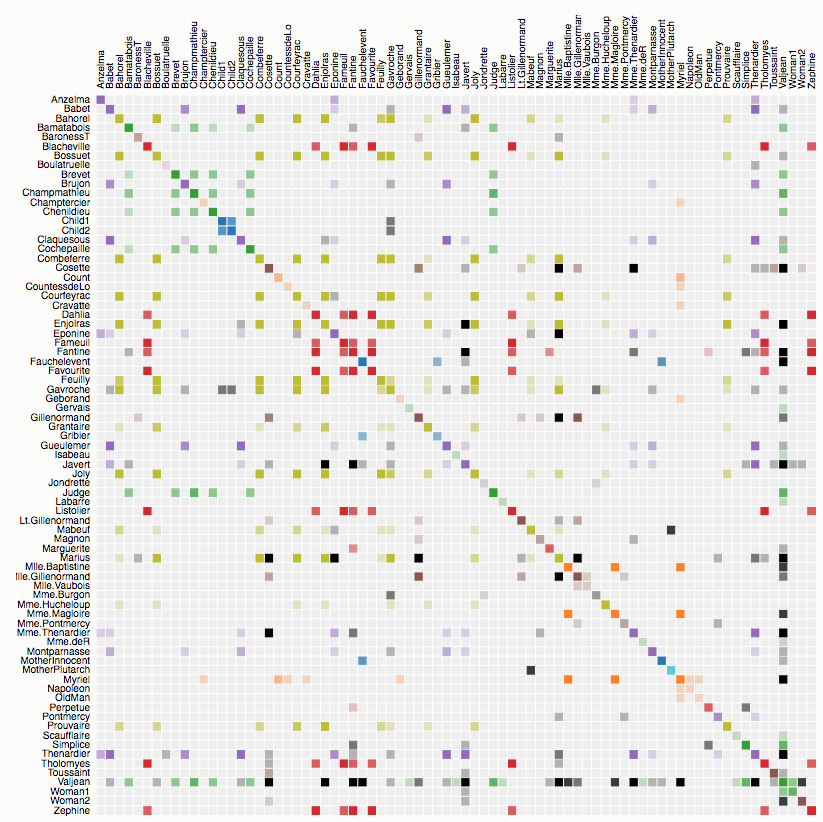
\includegraphics[width=\textwidth]{figures_c1/adja.png}
         \caption{Sorted by name}
         \label{fig:adja}
     \end{subfigure}
    %   \begin{subfigure}[b]{.32\textwidth}
    %      \centering
    %      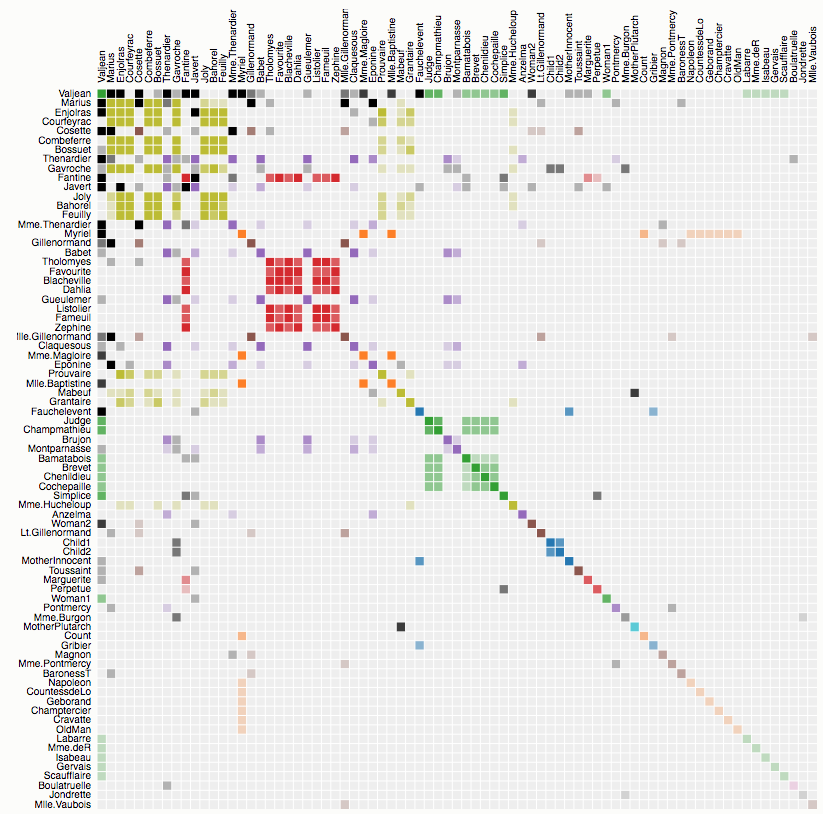
\includegraphics[width=\textwidth]{figures_c1/adjb.png}
    %      \caption{Sorted by degree.}
    %      \label{fig:adjpow}
    %  \end{subfigure}
            \begin{subfigure}[b]{.49\textwidth}
         \centering
         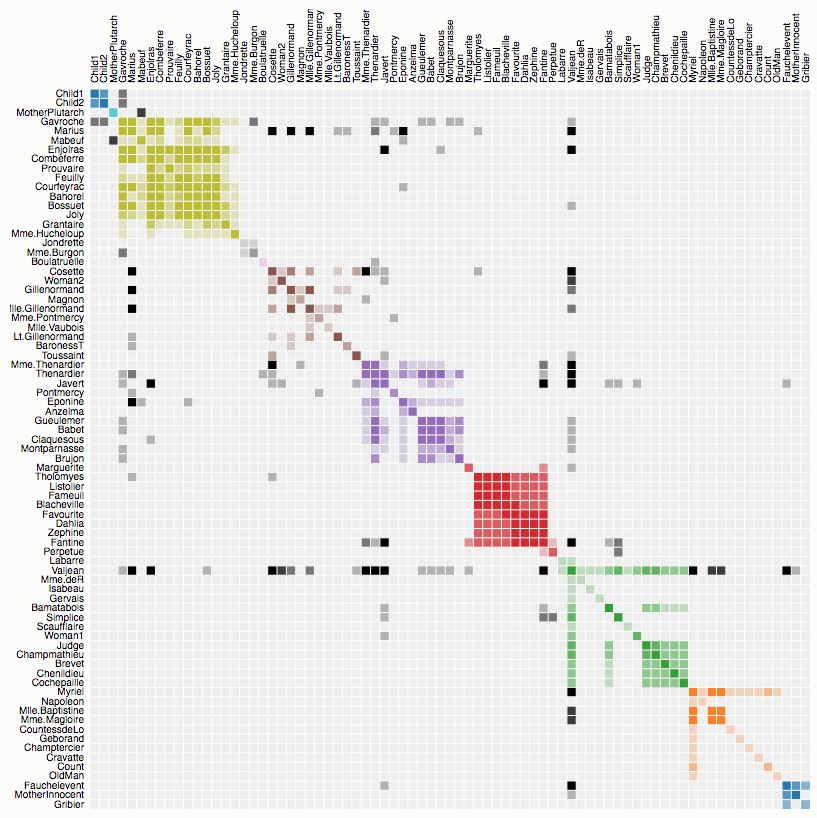
\includegraphics[width=\textwidth]{figures_c1/adjc.png}
         \caption{Sorted by cluster}
         \label{fig:adjclust}
     \end{subfigure}
        \caption{\textbf{The adjacency or relational matrix of the Les Miserables graph}. These show how changing the order of elements within a matrix can aid in the visual identification of clusters in the data. Squares features along the diagonal indicate a larger number of links between grouped items in the axis order, and less to those in other modules. Source: \citep{adj}}
        \label{fig:adj}
\end{figure}


\subsubsection*{Arc Diagrams}
Arc diagrams are a subset of sociographs where items are represented as nodes along the horizontal. Relationships between nodes are then shown through the use of curved links (arcs). It is this that makes them particularly suited for the highlighting of repetition between music or DNA sequences, \citep{arc}. Using the data as above I use an arc diagram to explore how species containing the same combination of functional groups react. This is done by first determining all branch permutations from the protocol flowchart (\autoref{fig:protocol}). This produces [179???????] groups which are positioned across the $x$ axis in ascending group size (the more branches matched, the further to the right a group is positioned). The width of each group is determined from the number of species within it. Next links are added between the species based on what groups the product species from each reaction contain. \autoref{fig:arcdiagram} discretizes reactions which produce products with an increased number of reaction pathways (positive arcs - top), from those which result in species with less (positive arcs - below). Here the cyclic nature of tropospheric chemistry can be seen, with many species producing larger, less stable, products, which then go on to react and dissociate back into smaller ones. In some cases a complete circle between two nodes can be indicative of a catalytic reaction.  Using interaction and selective shading, it is possible to isolate certain types of reactions and determine which of the functional groups are responsible for the change experienced within a reaction. 



\begin{figure}[H]
     \centering
     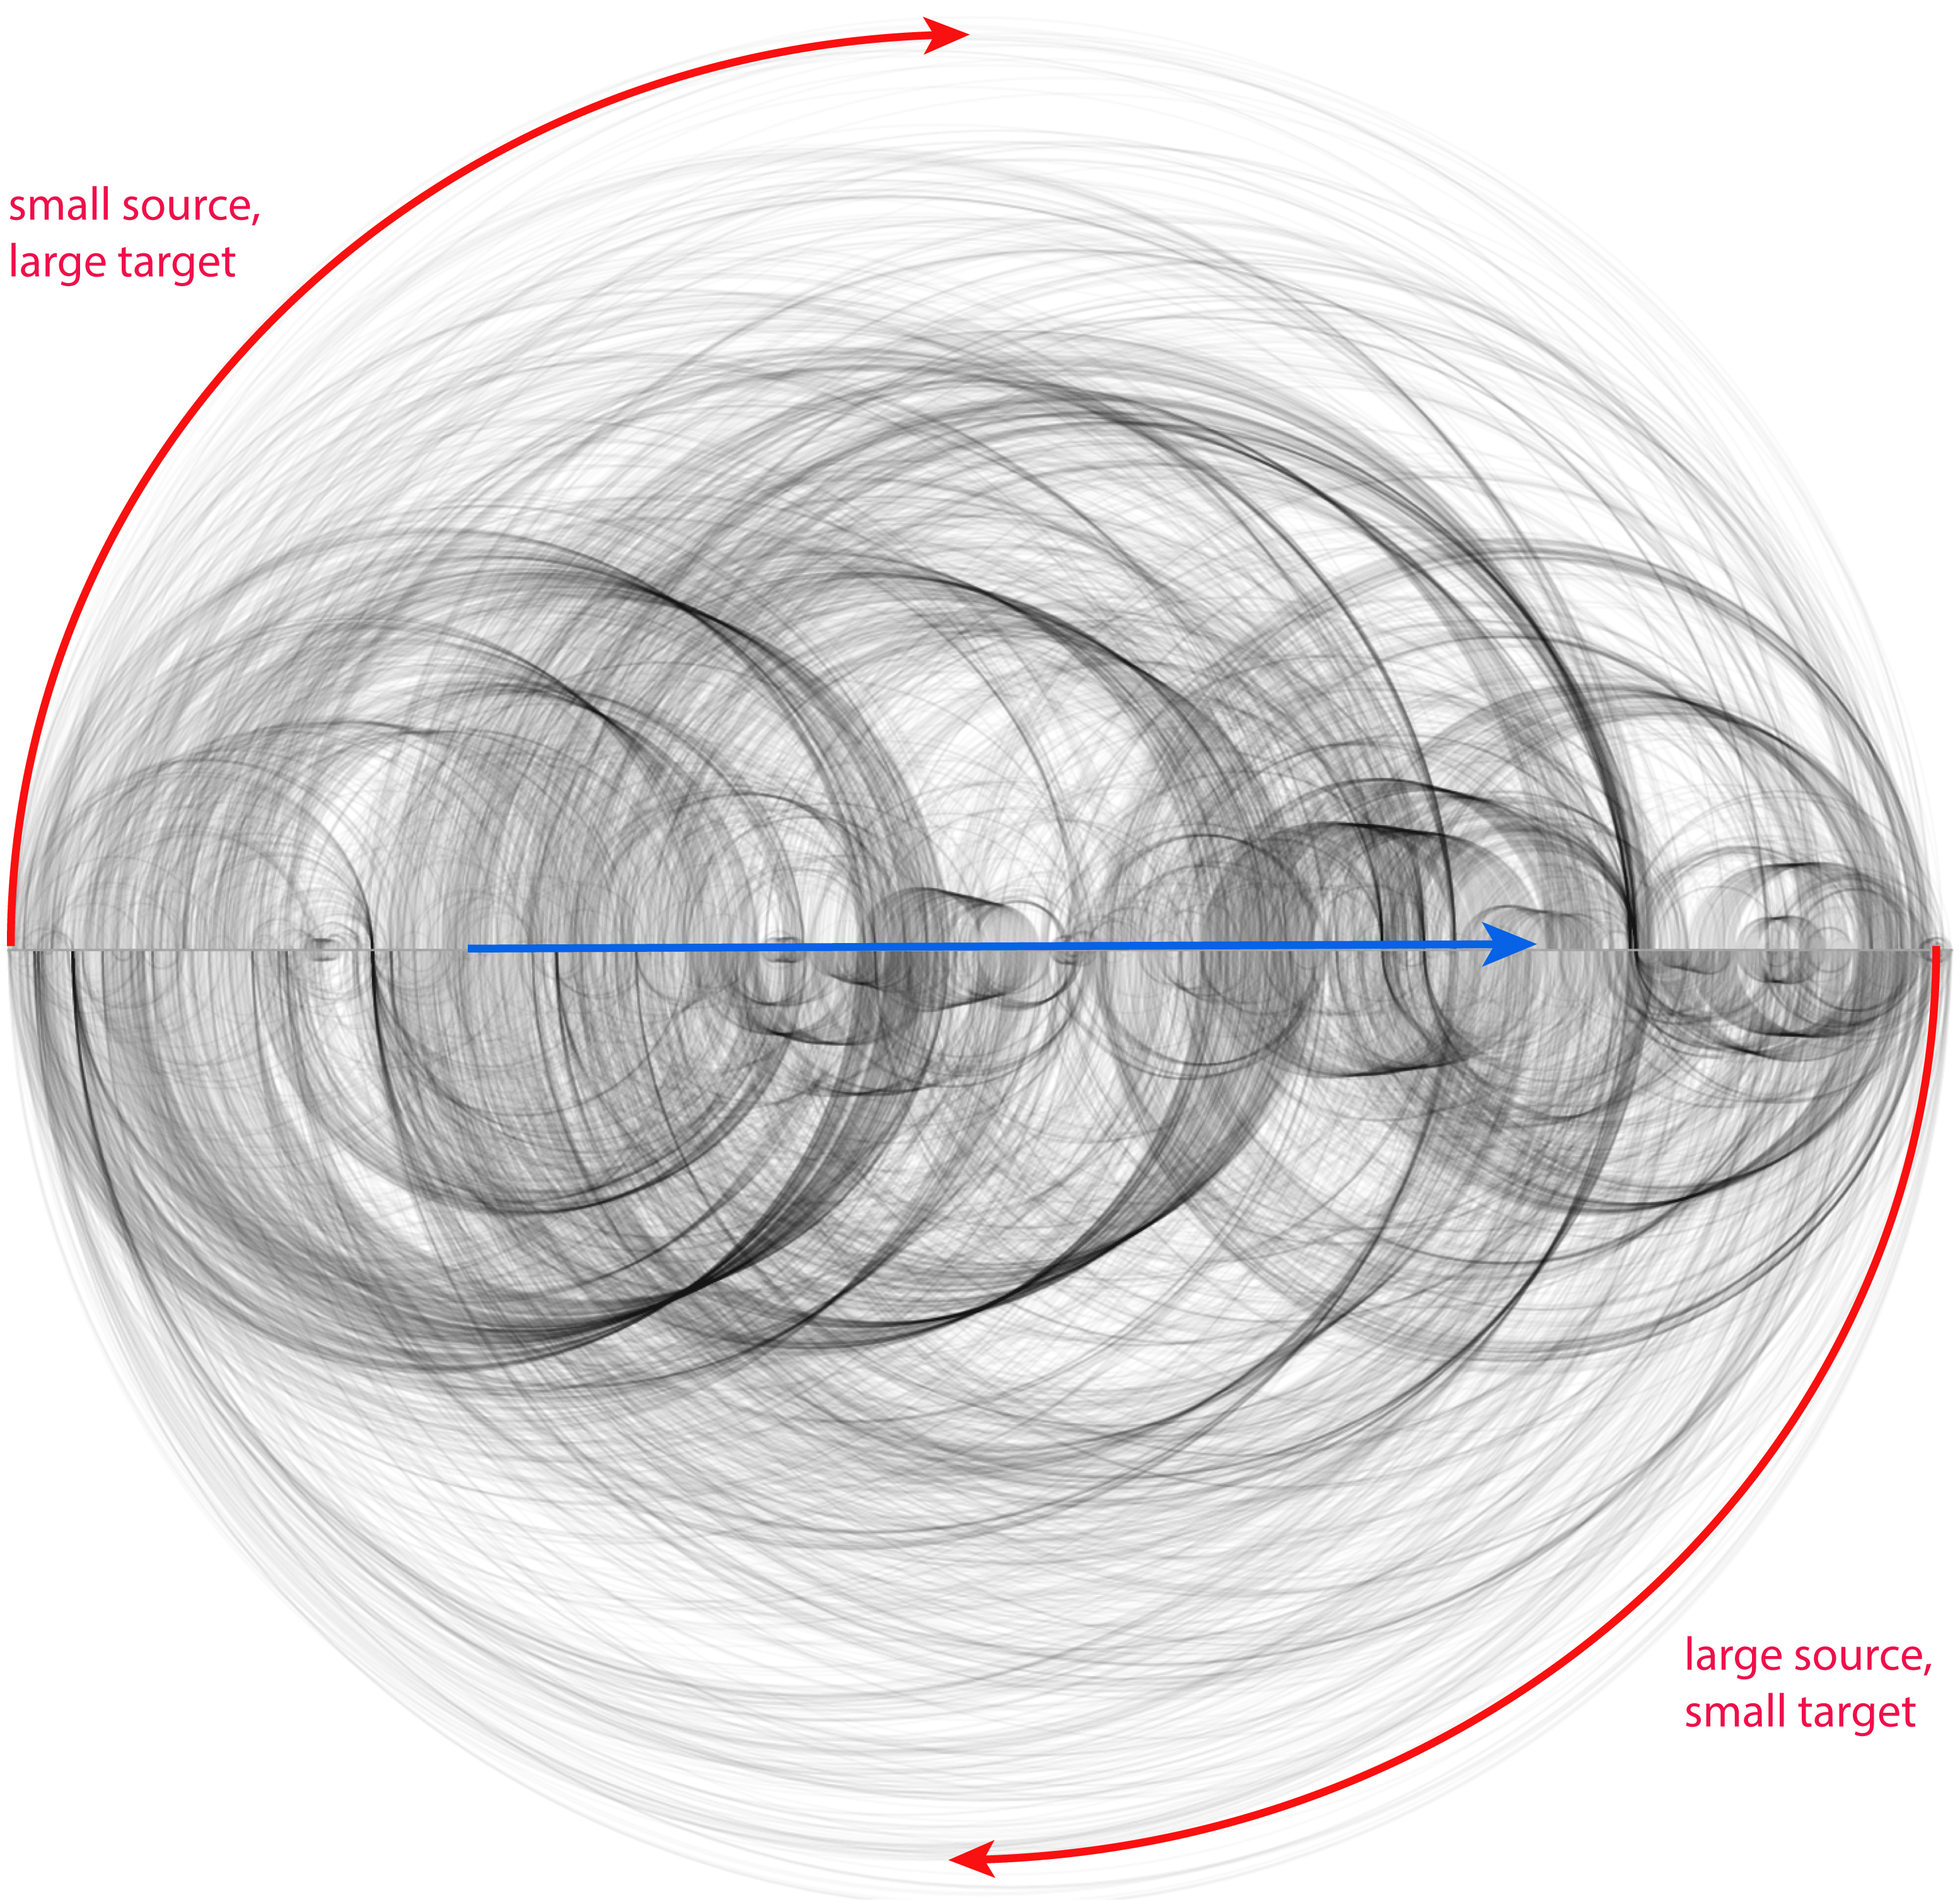
\includegraphics[width=.8\textwidth]{figures_c1/arc/arc_all.png}
     \caption{\textbf{An arc diagram constructed using the construction pathways presented in \autoref{fig:protocol}}. Possible pathways for each species are extracted. These are then grouped and sorted by the number of functional group/pathways available. Species are shown along the blue line and sorted with the most multifunctional groups to the right. Reaction pairs (reactant-product) are then depicted through the use of arcs. The direction of these is shown using the location of the arcs. }
     \label{fig:arcdiagram}
\end{figure}

Although such a layout may seem daunting at first, with many lines, in all directions, filtering by type of reactions can draw attention to several features from the chemistry. In REF CHAPTER/FIG the importance of $HO_x$ cycle for the removal of VOCs and greenhouse gasses is shown. For this reason, I decided to explore the relationship between reactions with OH and \ce{HO2}, \autoref{fig:ho2oh}. These are represented using individual versions of the complete arc plot, \autoref{fig:arcdiagram}, where the relevant reactions (i.e. containing the radical of choice) are the only ones highlighted in colour and increased in opacity, \autoref{fig:hv},\autoref{fig:oh}.  
Using this it is possible to see that several groups form arcs highlighting the cyclic OH $  rightleftharpoon HO_2 $ chemistry, 
\autoref{fig:rxnho2oh}. It is also visible that there are a significantly larger number of OH reactions, which corresponds to our knowledge of the mechanism, FIGURE MCM ALL. 

\begin{figure}[H]
     \centering
      \begin{subfigure}[b]{.4\textwidth}
         \centering
         \includegraphics[width=\textwidth]{figures_c1/arc/ho2oh.png}
         \caption{The most prominent branches. }
         \label{fig:hv}
     \end{subfigure}
      \begin{subfigure}[b]{.4\textwidth}
         \centering
            \scalebox{.7}{
        \schemestart [0,1,thick]
            \chemfig{R-[:-30](=[:-90]O)(-[:30]O-[:-30]O_{.})} 
             \arrow{->[\ce{HO2}][][][.5][]}
            \chemfig{R-[:-30](=[:-90]O)(-[:30]O-[:-30]OH)} 
            \arrow{0}[,0] \chemfig{\+ \ce{O2}}
         \schemestop\par    
     }\\ \ \\
    \scalebox{.7}{
        \schemestart [0,1,thick]
            \chemfig{R-[:-30](=[:-90]O)(-[:30]O-[:-30]OH)} 
            \arrow{->[\ce{OH}][][][.5][]}
            \chemfig{R-[:-30](=[:-90]O)(-[:30]O-[:-30]O_{.})} 
            \arrow{0}[,0] \chemfig{\+ \ce{H2O}}
         \schemestop\par    
         }\hfill
         \caption{Reactions observed}
         \label{fig:rxnho2oh}
     \end{subfigure}
     \begin{subfigure}[b]{.4\textwidth}
         \centering
         \includegraphics[width=\textwidth]{figures_c1/arc/ho2.png}
         \caption{\ce{Hydroxyl}}
         \label{fig:hv}
     \end{subfigure}
     \begin{subfigure}[b]{.4\textwidth}
         \centering
         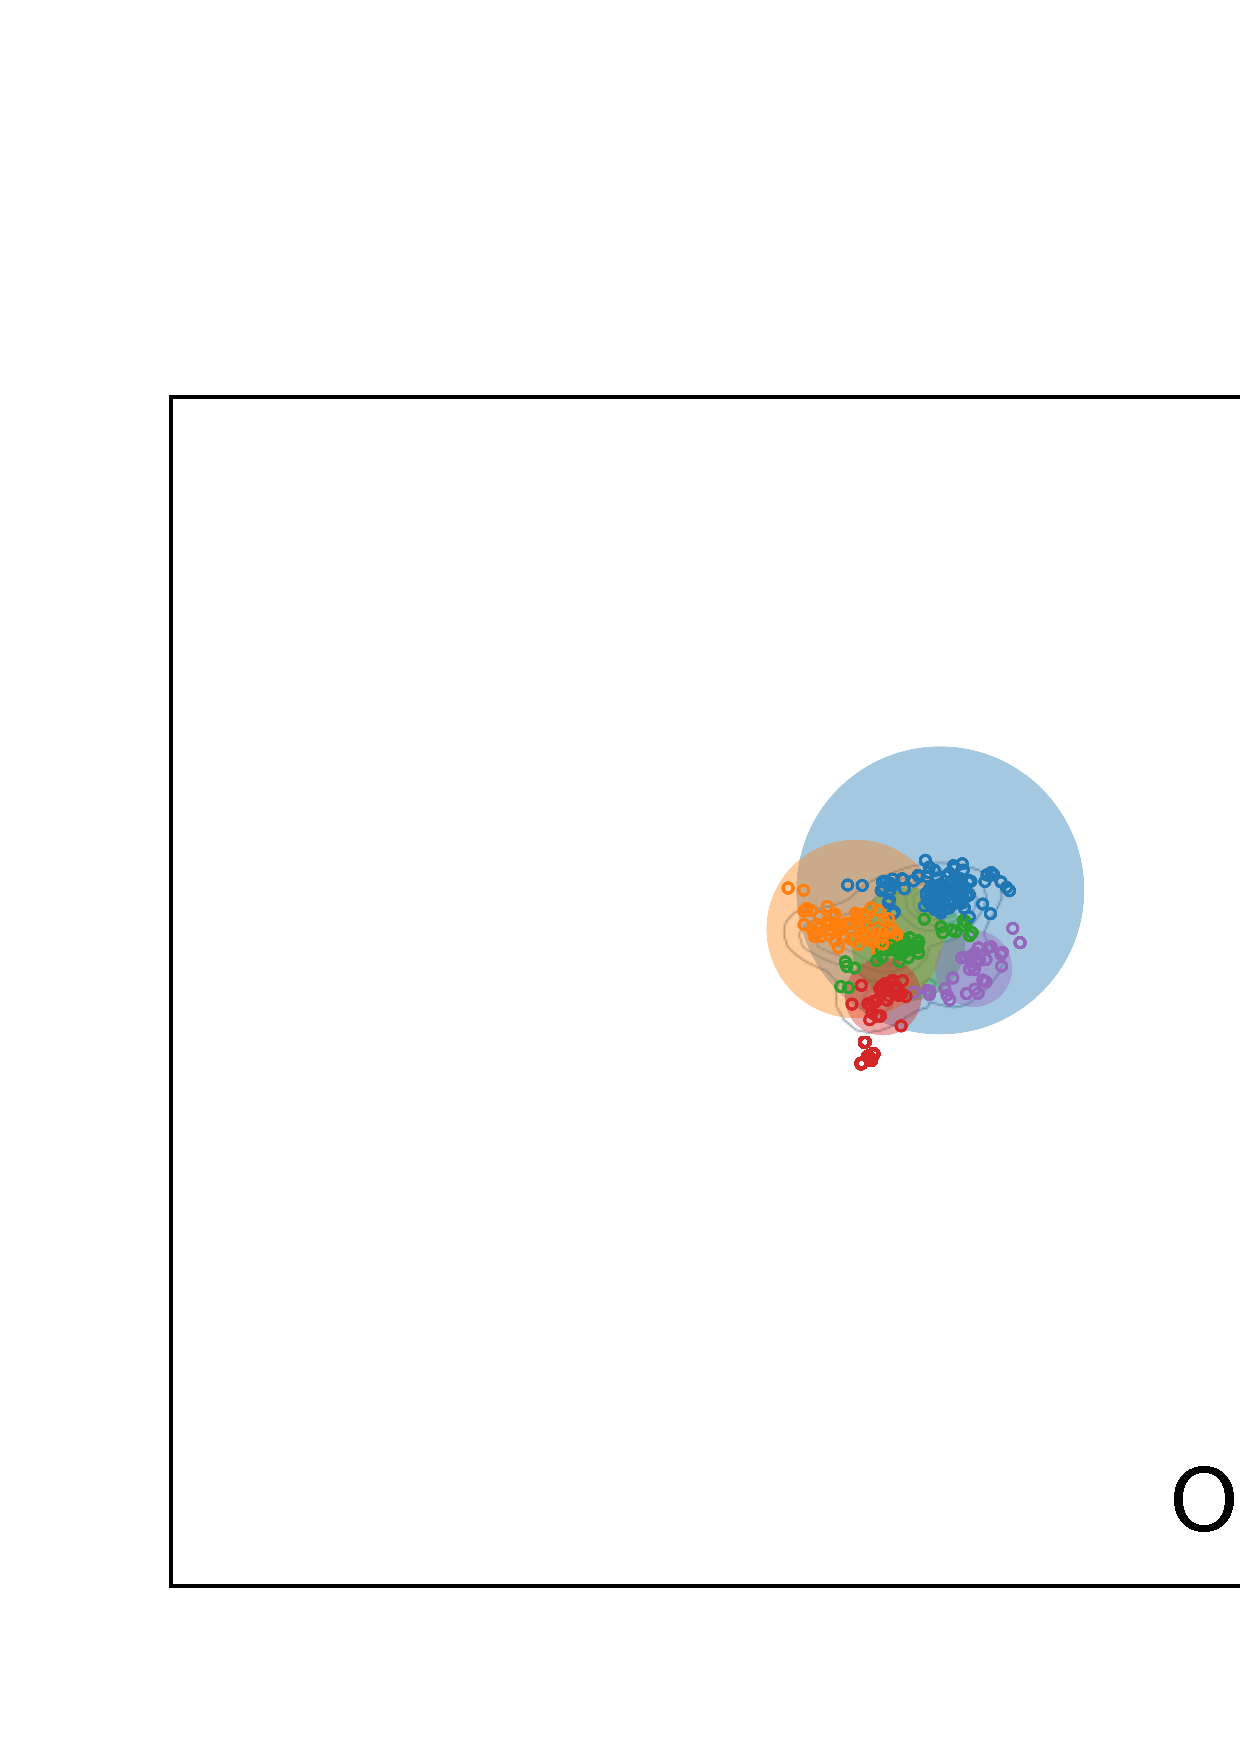
\includegraphics[width=\textwidth]{figures_c1/arc/OH.png}
         \caption{Hydroxide}
         \label{fig:oh}
     \end{subfigure}
      \caption{\textbf{ Arc diagram features for the Hydroperoxyl and Hydroxide radicals.} The $HO_x$ cycle chemistry (b) can ge seen within certain groups in the network. The main ones of these are hilighted in (a).   }
        \label{fig:ohho2}
\end{figure}


In addition to the reaction with the hydroxide radical, species may also be broken down with the aid of a photon - i.e. photolysis. If we compare all photolytic reactions, within those of OH, it can be seen that for certain groups, there exist two possible reaction pathways, \autoref{fig:rxnohhvv}. Since the reaction with OH serves to strip the hydrogen, the resultant species has a similar number of functional groups. Photolysis reactions, however, breaks the double bond, producing a species with a much smaller number of groups. This may be seen in the difference of length in the arcs emanating from these species, \autoref{fig:ohhv}. 




\begin{figure}[H]
     \centering
      \begin{subfigure}[b]{.4\textwidth}
         \centering
         \includegraphics[width=\textwidth]{figures_c1/arc/ohhv.png}
         \caption{The most prominent branches. }
         \label{fig:hv}
     \end{subfigure}
      \begin{subfigure}[b]{.4\textwidth}
         \centering
    \scalebox{.7}{
        \schemestart [0,1,thick]
            \subscheme{\chemfig{R-[:30](=[:90]O)-[:-30]O-[:30]OH} }
             \arrow(@c2--){->[$hv$]}[-25,1.8] 
              \chemfig{R-[:30]O-[:-30]O_{.}}
              \arrow{0}[,0] \chemfig{\+ \ce{HO2}}
              \arrow(@c2--){->[OH]}[20,1.8] 
              \chemfig{R-[:30](=[:90]O)-[:-30]O-[:30]O_{.}}
              \arrow{0}[,0] \chemfig{\+ \ce{H2O}}
         \schemestop\par    
         }\hfill
         \caption{Reactions observed}
         \label{fig:rxnohhv}
     \end{subfigure}
     \\ \ \\
     \begin{subfigure}[b]{.4\textwidth}
         \centering
         \includegraphics[width=\textwidth]{figures_c1/arc/hv.png}
         \caption{$hv$}
         \label{fig:hv}
     \end{subfigure}
     \begin{subfigure}[b]{.4\textwidth}
         \centering
         \includegraphics[width=\textwidth]{figures_c1/arc/OH2.png}
         \caption{Hydroxide}
         \label{fig:oh}
     \end{subfigure}
      \caption{\textbf{ Arc diagram features for photolysis and  hydroxide. reactions.  } Photolysis results in species with a reduced number of functional groups, and therefore longer arcs. OH reactions for the same species do not produce such a drastic change on group number, and therefore have a smaller arc lenght.}
        \label{fig:ohhv}
\end{figure}


Peroxy acetyl nitrates (PANs) play a key role in the modelling of photochemical smog (ozone events), \citep{pans}. PANs are species which are very stable a cold temperatures but can easily decompose and release $NO_x$ when warmed.
As this is an important species in the production of Ozone, this makes PANs an effective reservoir species with significant importance within atmospheric chemistry models (especially if transportation is involved). In the MCM the thermal decomposition of PANS is determined by the KBPAN rate constant. In comparing reactions of this, \autoref{fig:kbpans}, with those of \ce{NO2} (at rate KFPAN), the emergence of the species cycle is seen.  

\begin{figure}[H]
     \centering
      \begin{subfigure}[b]{.4\textwidth}
         \centering
         \includegraphics[width=\textwidth]{figures_c1/arc/pans.png}
         \caption{The most prominent branches. }
         \label{fig:pansdir}
     \end{subfigure}
      \begin{subfigure}[b]{.4\textwidth}
         \centering
            \scalebox{.7}{
        \schemestart [0,1,thick]
            \chemfig{R-[:30]O-[:-30]O-[:30]N(=[:90]O^{-})=[:-30]O} 
             \arrow{->[\ce{}][][][.5][]}
            \chemfig{R-[:30]O-[:-30]O_{.}} 
            \arrow{0}[,0] \chemfig{\+ \ce{NO2}}
         \schemestop\par    
     }\\ \ \\
    \scalebox{.7}{
        \schemestart [0,1,thick]
            \chemfig{R-[:30]O-[:-30]O_{.}} 
            \arrow{->[\ce{NO2}][][][.5][]}
            \chemfig{R-[:30]O-[:-30]O-[:30]N(=[:90]O^{-})=[:-30]O} 
         \schemestop\par    
         }\hfill
         \caption{Reactions observed}
         \label{fig:rxnpan}
     \end{subfigure}
     \begin{subfigure}[b]{.4\textwidth}
         \centering
         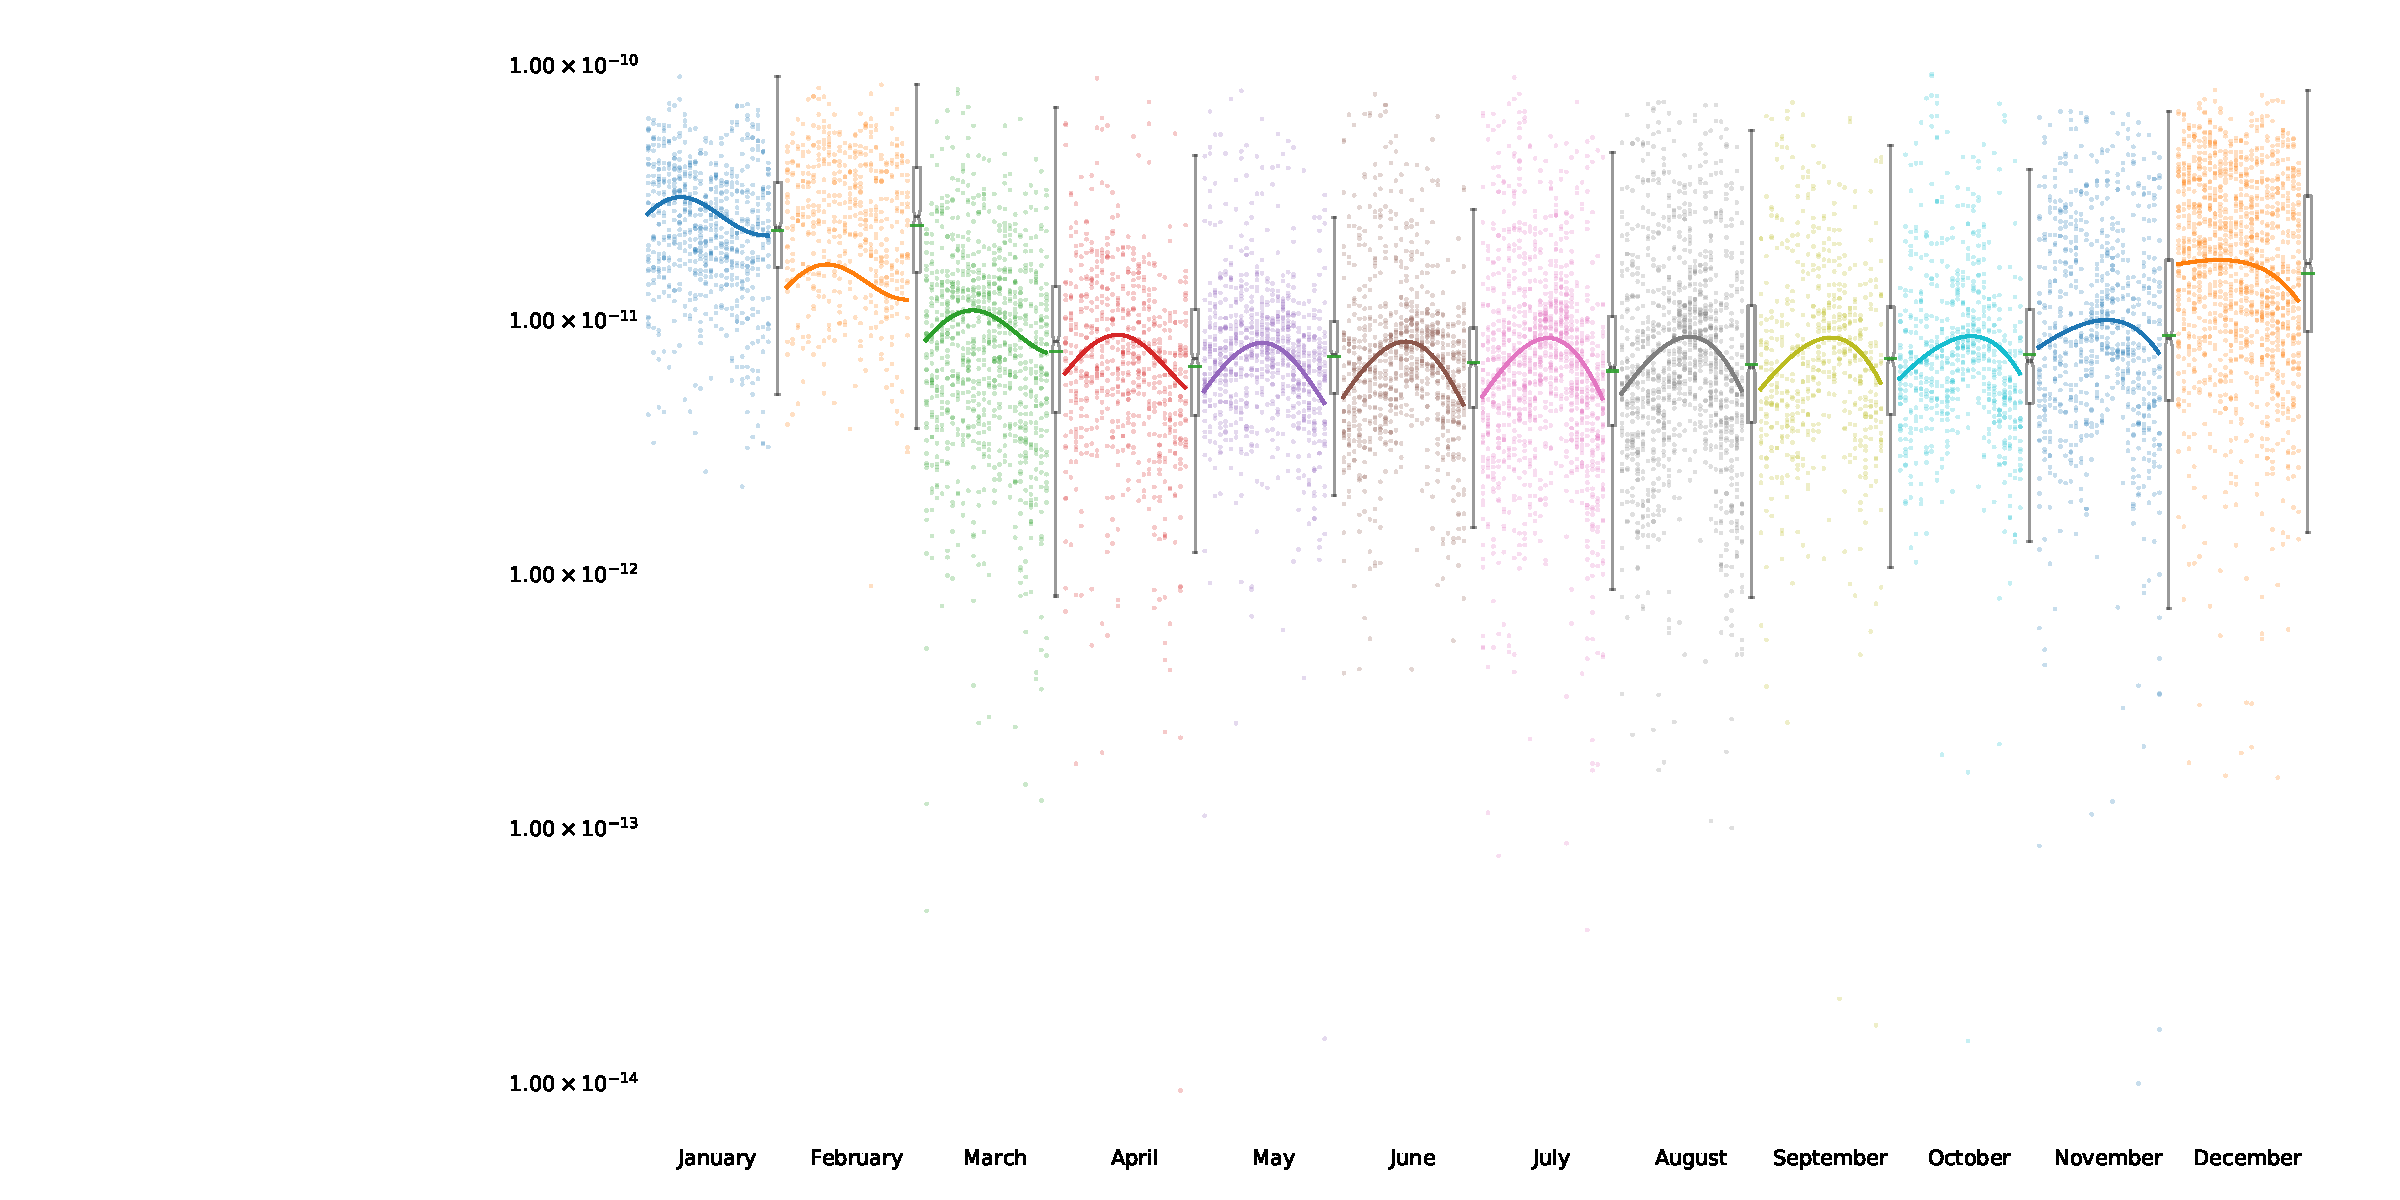
\includegraphics[width=\textwidth]{figures_c1/arc/NO2.png}
         \caption{\ce{NO2}}
         \label{fig:no2}
     \end{subfigure}
     \begin{subfigure}[b]{.4\textwidth}
         \centering
         \includegraphics[width=\textwidth]{figures_c1/arc/KBPAN.png}
         \caption{MCM reactions at the KBPAN rate.}
         \label{fig:kbpan}
     \end{subfigure}
      \caption{\textbf{ Arc diagram features for the PAN reactions. } }
        \label{fig:ohho2}
\end{figure}

Finally, patterns that exist within certain groups can be explored. We know that for \ce{RO2}-\ce{RO2} reactions there are three possible reaction pathways for the unpaired oxygen ... fill alter'


\textit{\textbf{NOTE:} A downside to the arc diagrams format that I have chosen is that for reactions between species of the same number of functional groups, there is no set direction. This can be seen in the positive arcs of  \autoref{fig:ro2}. }




\begin{figure}[H]
     \centering
      \begin{subfigure}[b]{.4\textwidth}
         \centering
         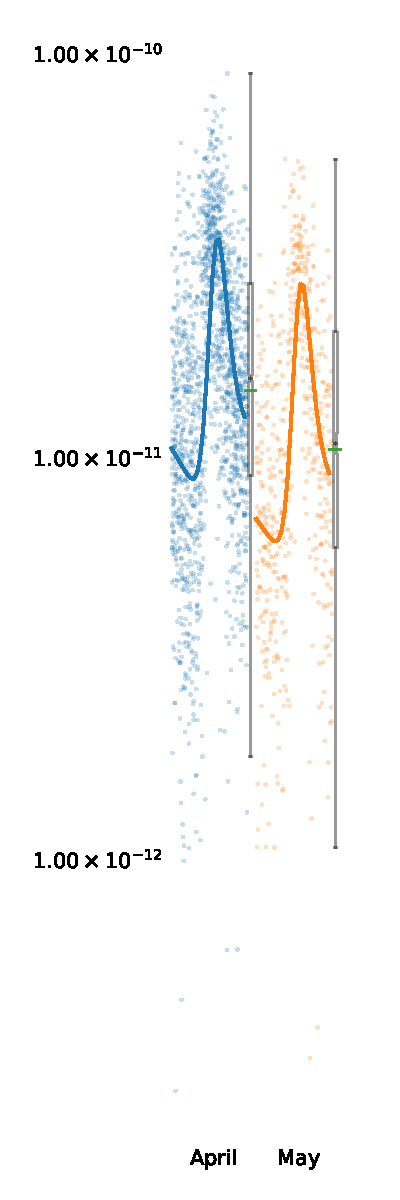
\includegraphics[width=\textwidth]{figures_c1/arc/RO2.png}
         \caption{\ce{RO2 - RO2} }
         \label{fig:ro2}
     \end{subfigure}
     \begin{subfigure}[b]{.4\textwidth}
        \centering
        \includegraphics[width=\textwidth]{figures_c1/arc/RO2HO2.png}
        \caption{\ce{RO2+HO2}}
        \label{fig:ro2ho2}
    \end{subfigure}
    \begin{subfigure}[b]{.4\textwidth}
       \centering
       \includegraphics[width=\textwidth]{figures_c1/arc/RO2NO.png}
       \caption{\ce{RO2+NO}}
       \label{fig:ro2no}
   \end{subfigure}
   \begin{subfigure}[b]{.4\textwidth}
      \centering
      \includegraphics[width=\textwidth]{figures_c1/arc/NO3.png}
      \caption{\ce{NO3} }
      \label{fig:no3}
  \end{subfigure}
\caption{\textbf{Categories with a net direction/trend.} It is possible to see the patterns in which certain reactions function.  }
  \label{fig:ro2arc}
\end{figure}



\subsubsection{The traditional network graph}

Finally, we have the traditional network representation in the form of a mathematical graph. 

Something about graphs. Intuitive. Blah


In \autoref{sec:netshape} it is shown that the network shape is constrained by the construction protocol of the MCM, and thus the chemistry it contains. In \autoref{graphplots} it is seen that in extracting an MCM subset to model different scenarios may result in the selection of sufficiently different mechanisms. This makes comparing the data collected difficult, as we do not know if a species' absence can be attributed to it having a very low concentration for a specific region, or simply that there was a lack of instrumentation capable of measuring it. A similarity in the mechanism subsets extracted as part of \autoref{fig:mace} (Mace Head) and \autoref{fig:london} (London) can be seen. Since both campaigns use a GC-FID (gas
chromatography with flame ionisation detection), \autoref{table:subsetsize} the similarities in recorded species may be in-part attributed to this. Beyond the instrumentation, it the ClearFlo (London) campaign measures the most long-chain hydrocarbons; Mace Head records the most benzine based species possibly due to shipping emissions and Borneo (\autoref{fig:borneo}) has the most terpene species - it is a rainforest. 



\begin{table}[H]
\begin{tabular}{l|llll}
                   & Full MCM   & Mace Head      & London      & Borneo        \\ \hline
Species            & XXXX       & 2363           & 1857        & 1587          \\
Instrument            & n/a       & GC-FID           &   DC-GC-FID and\\ GC$\times$GC-FID      & FAGE          \\
Observation Source & \citep{mcm} & \citep{lewis97} & \citep{clfo}\\\citep{dunmore} & \citep{borneo}\\
\end{tabular}
\caption{\textbf{The subset sizes, campaigns and instrumentation used for measurement.}}
\label{table:subsetsize}
\end{table}



\begin{figure}[H]
     \centering     
      \begin{subfigure}[b]{0.495\textwidth}
         \centering
         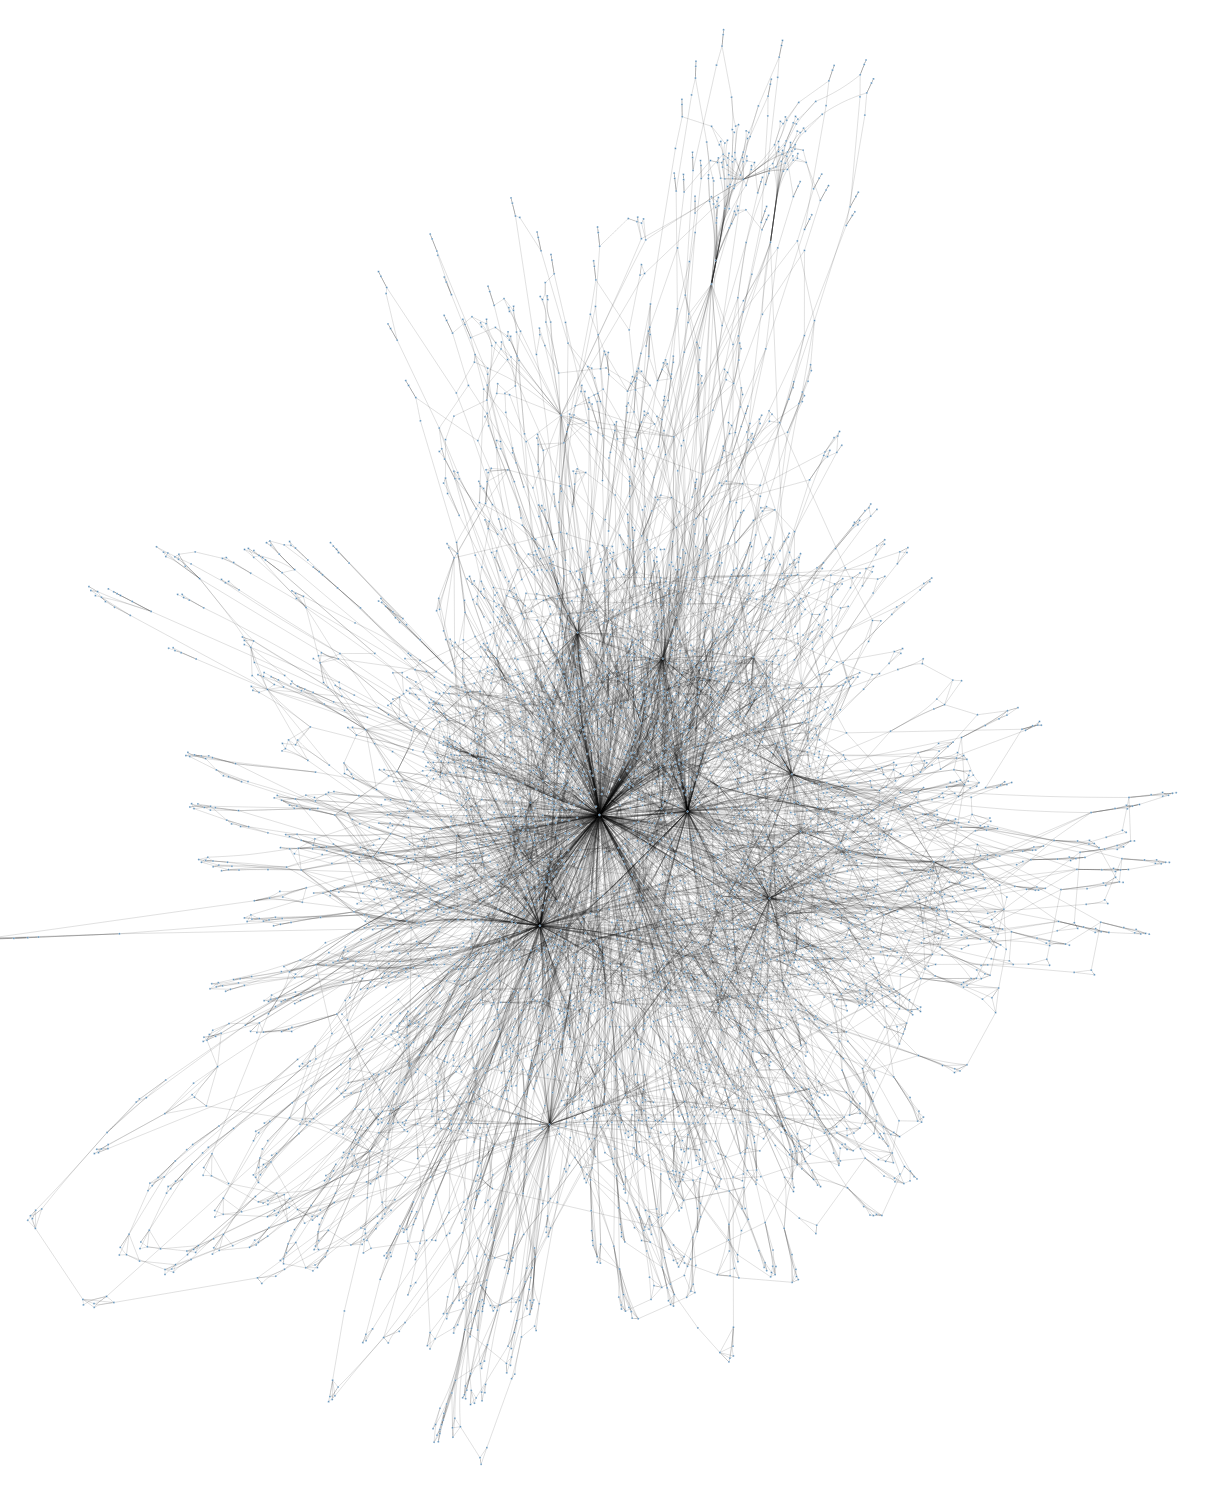
\includegraphics[width=\textwidth]{figures_c1/graph_compare/fullmcm.png}
         \caption{The full MCM (v3.3.1)}
         \label{fig:mcm}
     \end{subfigure}
      \hfill
       \begin{subfigure}[b]{0.495\textwidth}
          \centering
          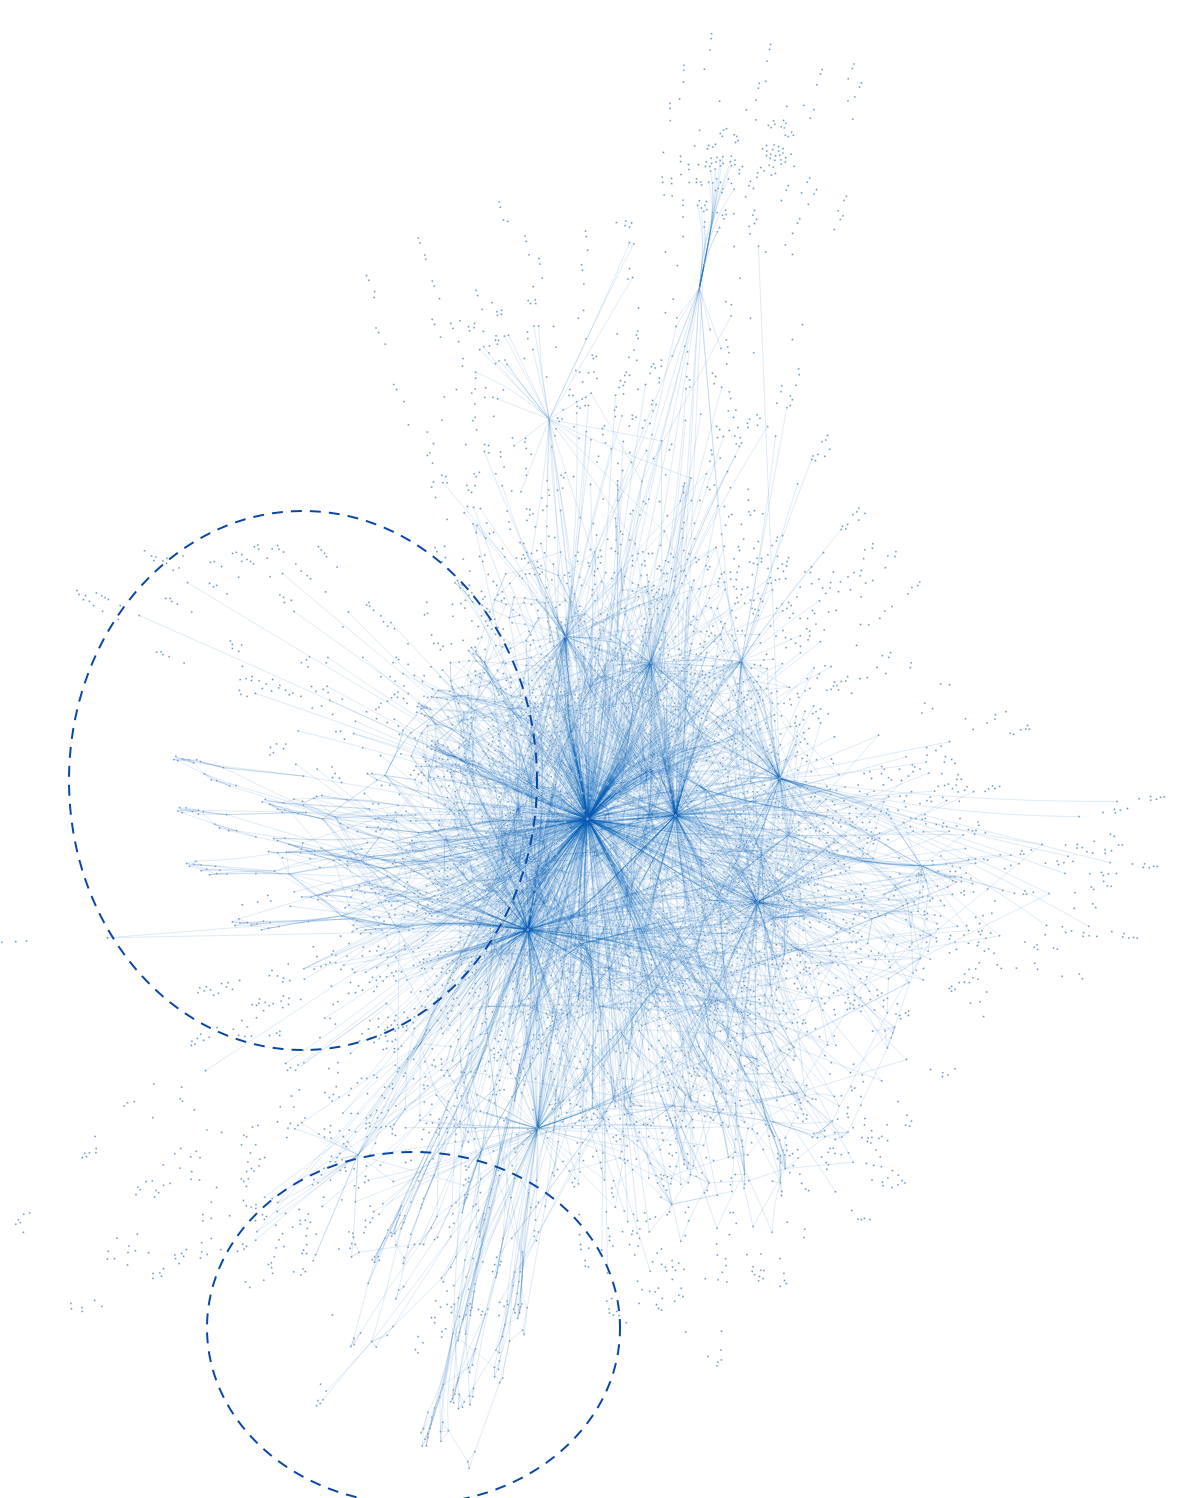
\includegraphics[width=\textwidth]{figures_c1/graph_compare/borneo.png}
          \caption{MCM subset of Borneo}
          \label{fig:borneo}
      \end{subfigure}
      \hfill
       \begin{subfigure}[b]{0.495\textwidth}
          \centering
          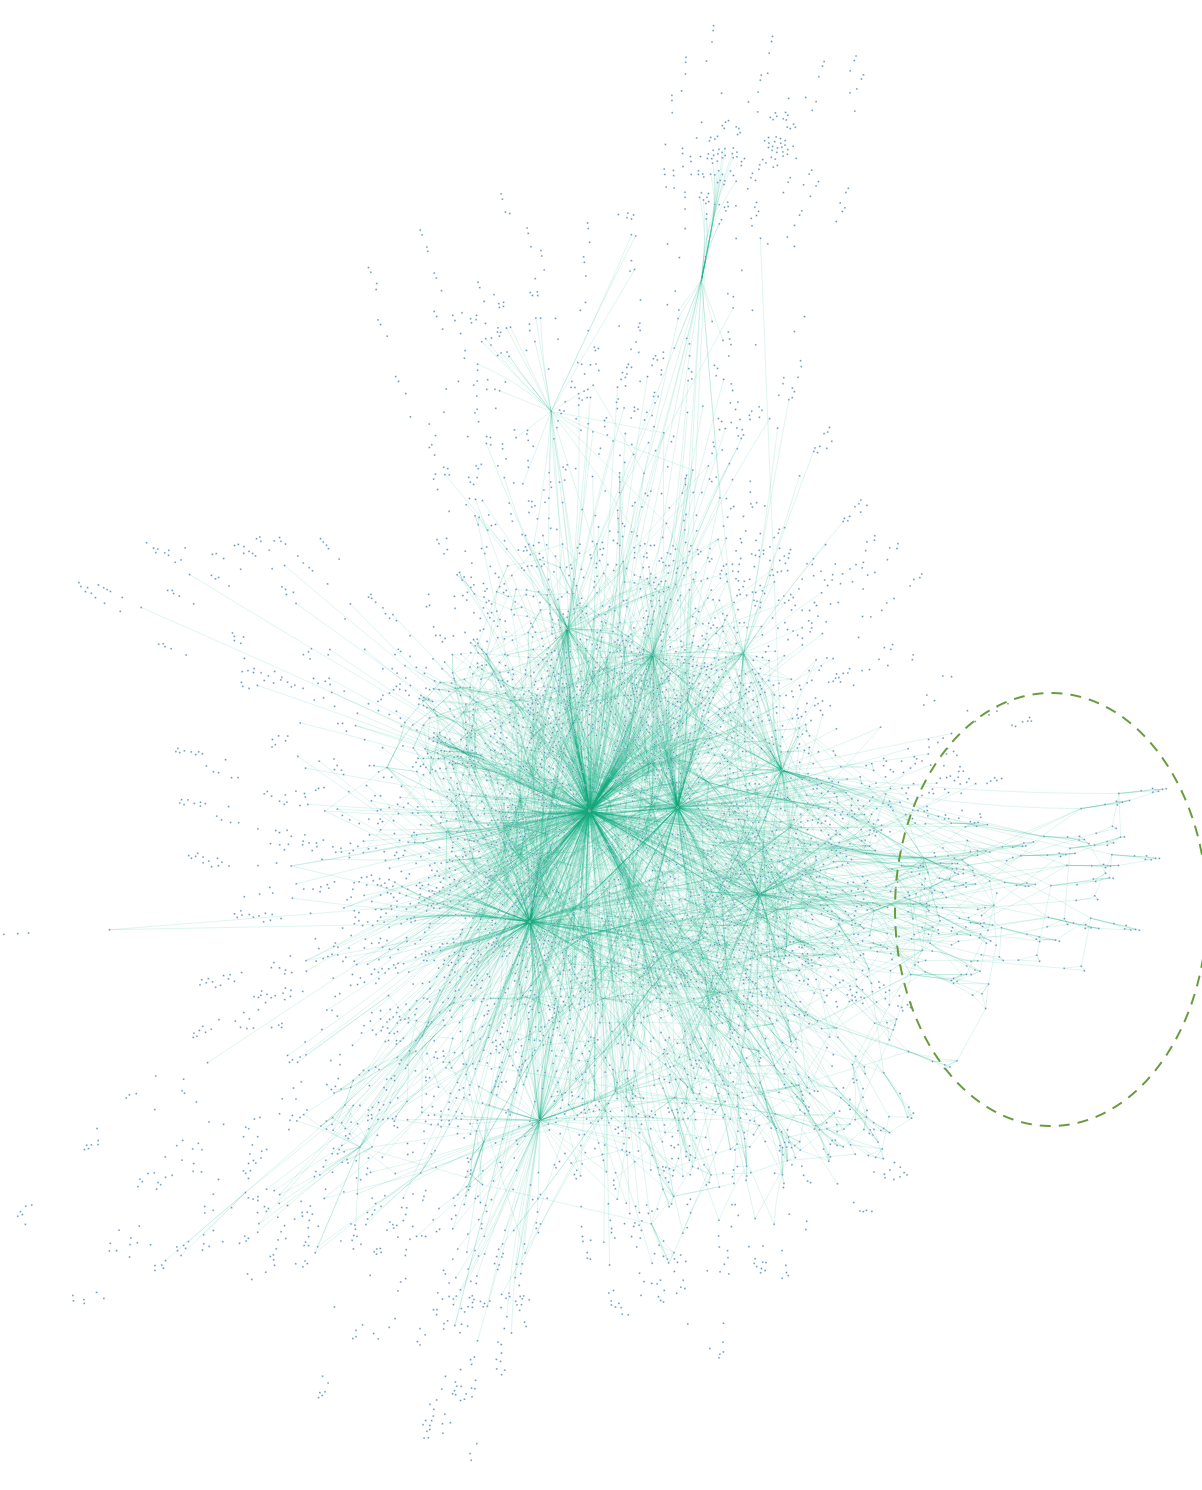
\includegraphics[width=\textwidth]{figures_c1/graph_compare/london.png}
          \caption{MCM subset of London}
          \label{fig:london}
      \end{subfigure}
       \hfill
        \begin{subfigure}[b]{0.495\textwidth}
           \centering
           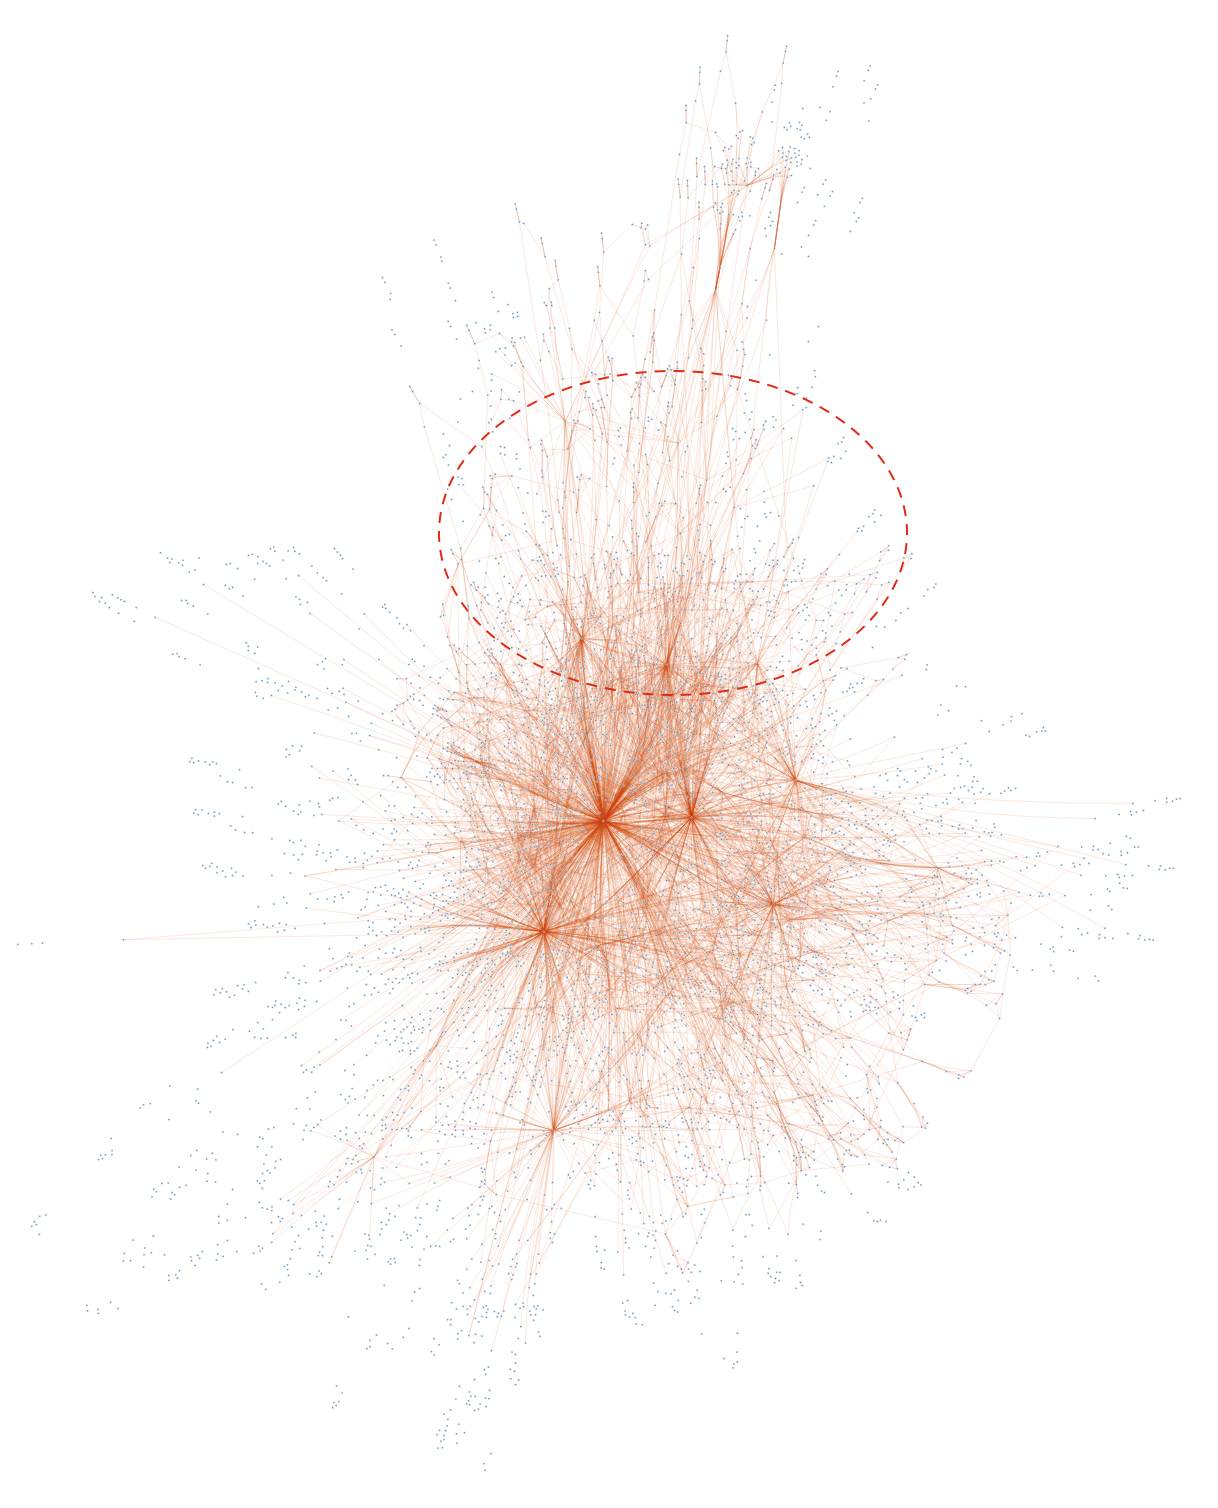
\includegraphics[width=\textwidth]{figures_c1/graph_compare/macehead.png}
           \caption{MCM subset of Mace head}
           \label{fig:macehead}
       \end{subfigure}
        \caption{\textbf{Comparing MCM subsets using the traditional graph representation.} A graph (a) for the whole MCM is created. From this several mechanism subsets are extracted. The species and reactions are then extracted to produce the plots (b-d). All the species within the MCM are shown for comparion between plots, with only the links relevant to the mechananism being coloured.   }
        \label{fig:graphplots}
\end{figure}







\subsection{Summary}
Several different visualisation methods have been suggested. [select get filter statemen: donald knuth?]

Although each holds a different strength, node-link style methods tend to prevail in the representation of complex relationships for large systems. Other methods such as the chord diagram, tend to require a greater amount of pre-processing, which can obfuscates certain parts of the data. Matrix representation methods, although great for applying algorithms to, can often prove problematic for very large or sparse networks. Additionally these generally only have a single relationship between two items, meaning that information has to be grouped or averaged before use. Node-Link methods can not only allow easy filtration, by interactively hiding edges or reducing their opacity, but they show the entire state of the network, enabling to make informed choices about which parts are suitable for further exploration. Finally, the physical notion of a thread binding two items is intuitive and simple to comprehend, making these graph-like structures the perfect metaphor for representing relationships within the real world. 

